\section{RF analysis}

At each session's end, a RF analysis was held to assess whether the V1 imaged position corresponded to neurons with RFs centred in the center of the visual field, as these were the fixed intended positions for the subsequent SM spatial structure analysis.

Responses of each ROI were baseline subtracted and analysed trial by trial, mapping each trial's response to the visual field position that the corresponding stimulus was presented at (figure \ref{rfanalysis}, left panels).

Then, these responses were averaged over repetition trials, portraying mean response levels for each of the visual field positions (figure \ref{rfanalysis}, middle panels).

Finally, normalized gray-scale maps were produced for the response maps $R(az, el)$, with $az$ and $el$ the azimuth and elevation retinotopic coordinates, averaging over time on each of the positions' mean trace responses (figure \ref{rfanalysis}, right panels).

\begin{figure}[H] \centering 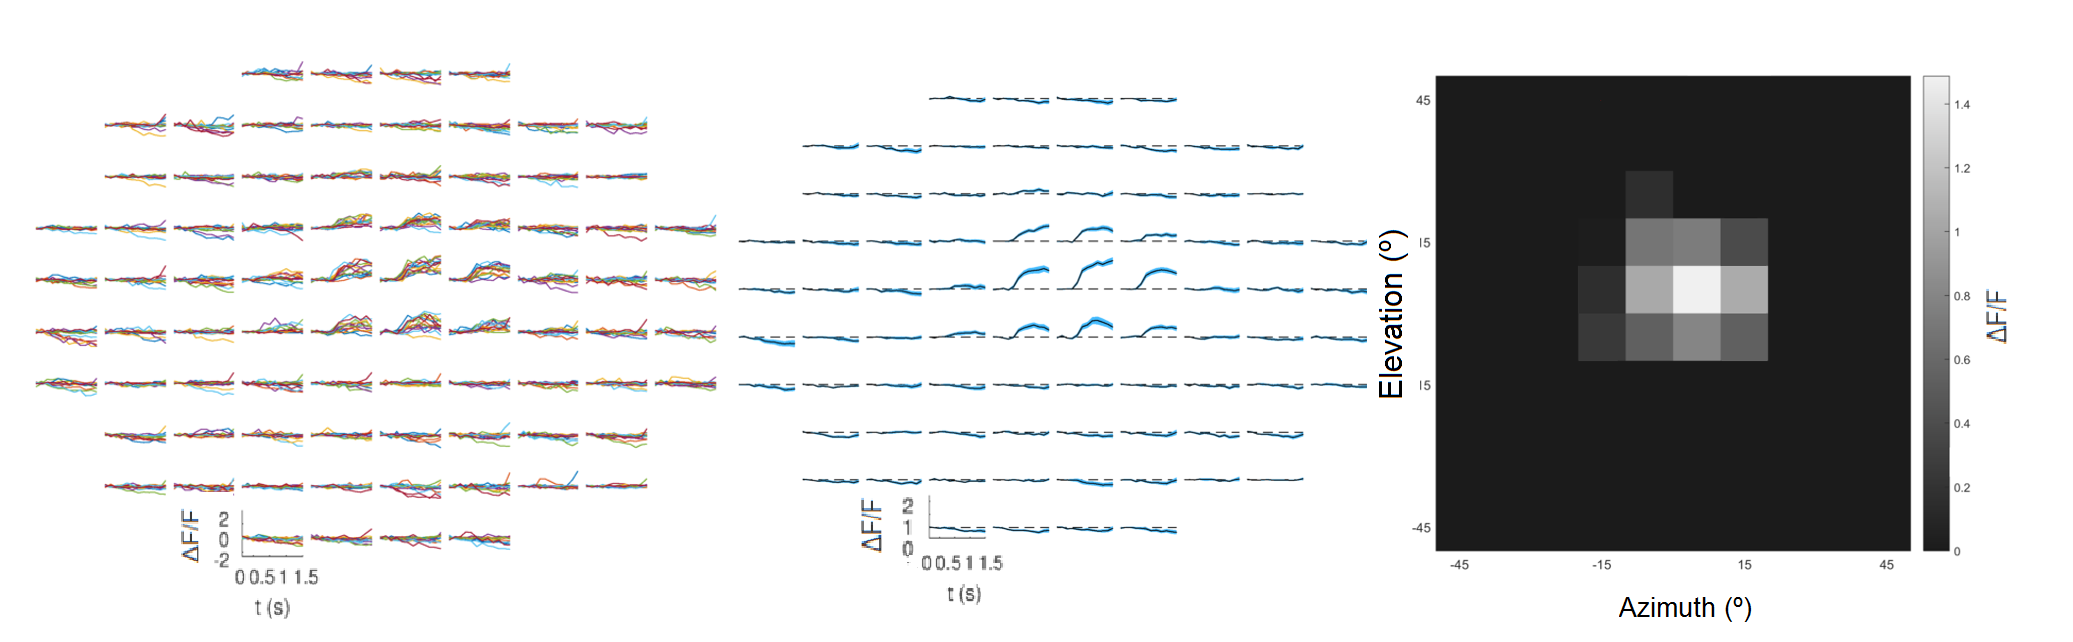
\includegraphics[width=13cm,height=13cm,keepaspectratio]{Figures/7.Results/rf/rf1.png} 
\caption{Example cell with well centred RF. 
\newline \textbf{Left:} Individual traces. Each of the 14 trial-type repetition trace response is represented in a different colour, for each of the visual field stimulated region. 
\newline \textbf{Middle:} Mean traces. Average traces over the 14 repetitions, represented also for each azimuth and elevation center stimulus condition. 
\newline \textbf{Right:}RF map. Response strengths to each of the stimulus positions, in a gray-scaled colour map.}
\label{rfanalysis}
\end{figure}

Each of these neurons' response maps was fitted to 2D-Gaussian ellipses, using Matlab implementation of the least-squares Levenberg-Marquardt algorithm (as in \cite{Marques2018}):

\begin{dmath}
R(az,el)=a+b\times \exp \left[ - \left( \dfrac{az-az_0}\times \cos(\theta)+ el-el_0)\times \sin(\theta){\sqrt{2} \times \sigma_1}\right)^2 - \left( \dfrac{-(az-az_0) \times sin \theta + (el-el_0)\times \cos(\theta)}{\sqrt{2} \times \sigma_2}\right)^2\right]
\end{dmath}

with $(az_0, el_0)$ the 2D Gaussian center coordinates, $\sigma_1$ and $\sigma_2$ the standard deviations of the gaussian across the two dimensions, $\theta$ the rotation angle between the gaussian and the $(az,el)$ axis, $a$ an offset parameter and $b$ an amplitude parameter.

The RF was then defined as the ellipse centred at $(az_0, ele_0)$ and limited by the standard deviations  ($\sigma_1$, $\sigma_2$):

\begin{equation}
\left[ \left( \dfrac{(az-az_0)\cdot \cos(\theta) + (el-el_0)\cdot \sin(\theta)}{\sigma_1}\right)^2 + \left(\dfrac{-(az-az_0)\cdot \sin(\theta) + (el-el_0)\cdot \cos(\theta)}{\sigma_2}\right)^2\right]=1
\end{equation}

The subsequent analysis was restricted to fits with $R^2>0.5$, as lower values corresponded to RF unreliable estimations. Within 10 sessions with 4 planes each, across 4 animals, 3168 out of 4198 dataset ROIs ($75\%$) were considered.

Analysing plane by plane, for each animal and session (example planes in figure \ref{ellipses}), one could assess that most of the considered RF centres were placed with similar centres within the retinotopical space, as theoretically expected for the short distances of $200 \times 200) \mu m$ imaged V1 planes. 

Two of the sessions showed very high elevation RFs, and were thus discarded for subsequent analysis, leaving 2772 measured RF cells and a total of 3728 cells ($74\%$ fitted RFs) to be analysed in regards to SM effects.

\begin{figure}[H] \centering 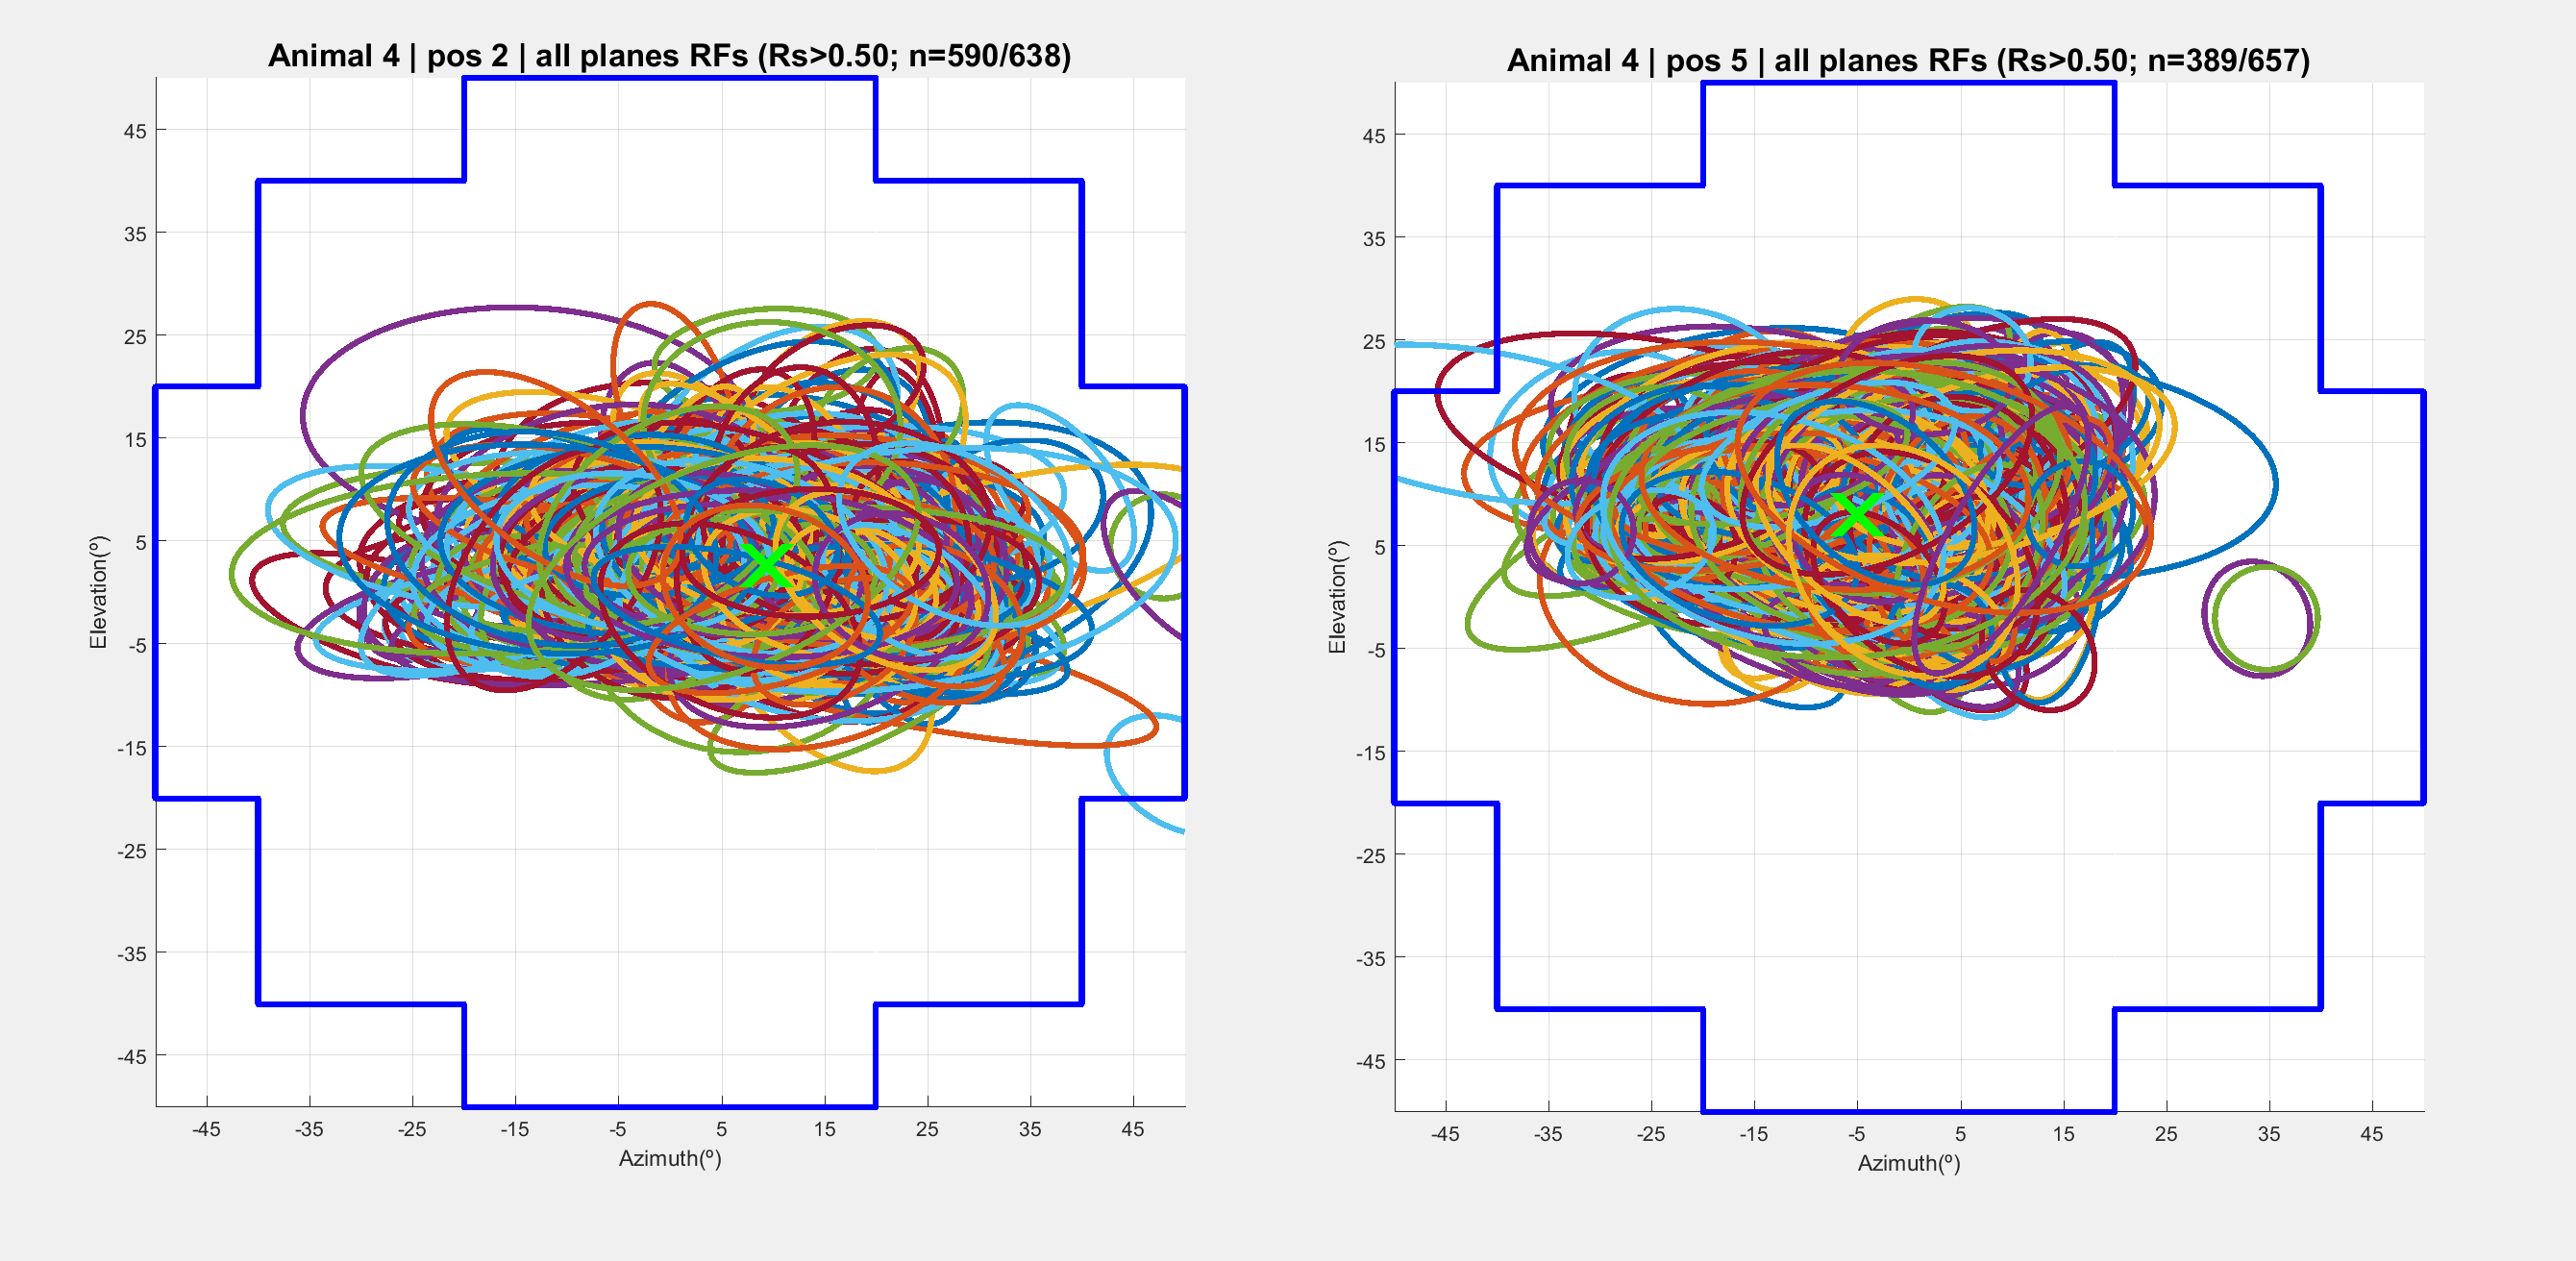
\includegraphics[width=13cm,height=13cm,keepaspectratio]{Figures/7.Results/rf/ellipsesAnimal4pos2andpos5.png} 
\caption{Superimposed 2D gaussian ellipsoidal fits for each neuron in the same plane. Two planes from two different sessions with the same animal are presented as examples.}
\label{ellipses}
\end{figure}

\section{Tuning analysis}
\label{tuningresults}

To validate bpod's tuning protocol, the selected neurons were analysed in regards to their direction (8 directions), spatial (2) and temporal (2) frequencies tuning selectivity.

Neurons in V1 can have orientation selectivity (\cite{Hubel1959}, \cite{Hubel1962}), that is, respond more strongly to a preferred orientation than to any other orientation. For mice, these orientation-selective (OS) cells are not organized into functional columns as they are for carnivores and primates (\cite{Hubel1962}, \cite{Hubel1968}), yet they do present strong orientation selectivity (\cite{Girman1999}, \cite{Ohki2005}). 

Moreover, a subset of  OS cells are also direction-selective (DS): these respond most strongly to a preferred direction than to any other.

For orientation analysis, responses of opposite directions are averaged together, and ploted on polar coordinates (figures \ref{tuninganalysisOS} and \ref{tuninganalysisDS}). The vector sum of responses at each individual trial (combining the trials for each of the same orientation opposed directions) then forms the \textit{orientation vector} of that trial. The orientation vectors for all trials then exhibit the cell's orientation tuning properties.
In the analogous way, for direction analysis, each trial measurement is binned to different direction labels, and the vector sum of the responses at individual directions then amounts to a direction vector for each trial. Direction vectors for all trials represent the cell's direction tuning properties.

Statistical significance is assessed with vector-based Hotelling's $t^2$-tests with confidence of 95\% in this project's case, as suggested by examinations in \cite{Mazurek2014}, to ask whether the 2D mean of the distribution of orientation and or direction vectors differ from (0,0).
 
 For any orientation, if the responses to a given orientation are significantly higher than responses to any other orientation, then the former is called the neuron's preferred orientation. This differential effect can be measured with an orientation selectivity index (OSI), for the preferred orientation response in the considered space. With  $R_{pref_or}$ the responses to the preferred orientation and $R_{orth}$ the responses to the orientation orthogonal to the preferred:
\begin{equation}
\text{OSI}= \dfrac{R_{pref \_or} - R_{orth}}{R_{pref \_or} + R_{orth}}
\end{equation}

Similarly, in the direction space, a preferred direction can also be determined for neurons that have significantly higher responses in one direction than they do in the null direction relative to the former. A DSI can be computed, for the direction doublet:

\begin{equation}
\text{DSI}=\dfrac{R_{pref} - R_{null}}{R_{pref} + R_{null}}
\end{equation}

In regards to the spatial and frequency tuning, here we used a restricted $(2 \times 2)$ space and found as expected (\cite{Whichpapershowsthis?}) that for most cells, in this space, the preferred spatial frequency was of 0.04 cycles per degree and the preferred temporal frequency was at 1 Hz. These were the frequency specifications used in both the RF protocol and the SM protocol.

Here, we present two example cell responses for the different stimulus conditions in the tuning protocol: an OS cell (figure \ref{tuninganalysisOS}) and a DS cell (figure \ref{tuninganalysisDS}).

\begin{figure}[H] \centering 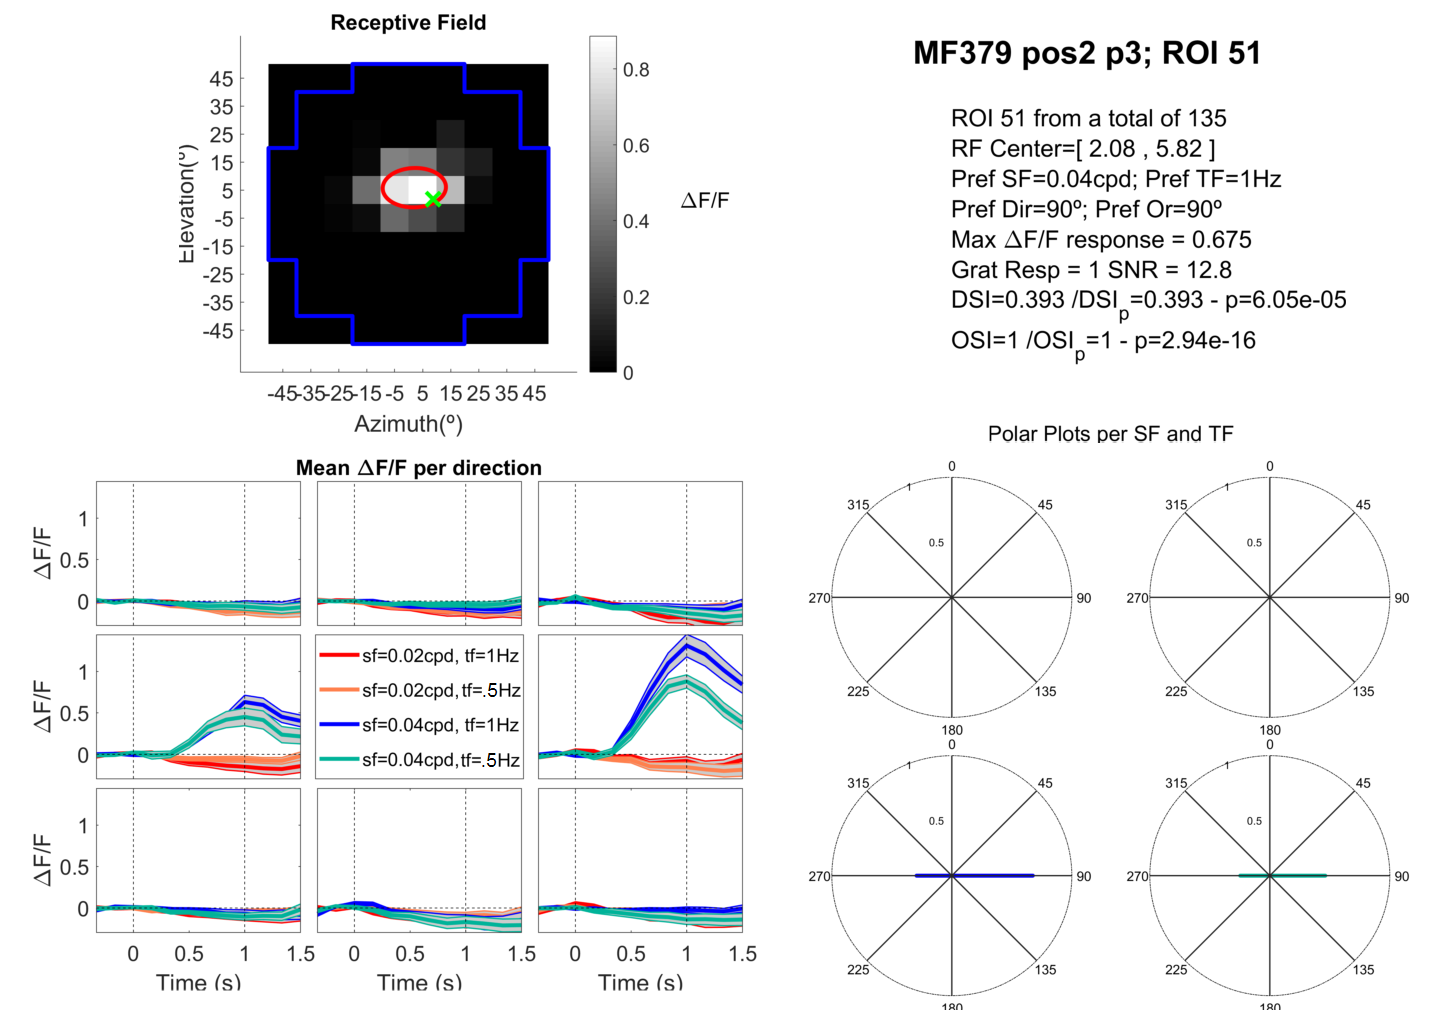
\includegraphics[width=12cm,height=12cm,keepaspectratio]{Figures/7.Results/tuning/MF379_pos2_p3_ROI0051.png} 
\caption{Tuning analysis for an example OS cell. Preferred $SF=0.04 cpd$, $TF=1 Hz$, up direction and vertical orientation. $DSI=1$ ($p=1.87 \cdot 10^{-5}$), $OSI=0.967$ ($p=3.4 \cdot 10^{-4}$).}
\label{tuninganalysisOS}
\end{figure}

\begin{figure}[H] \centering 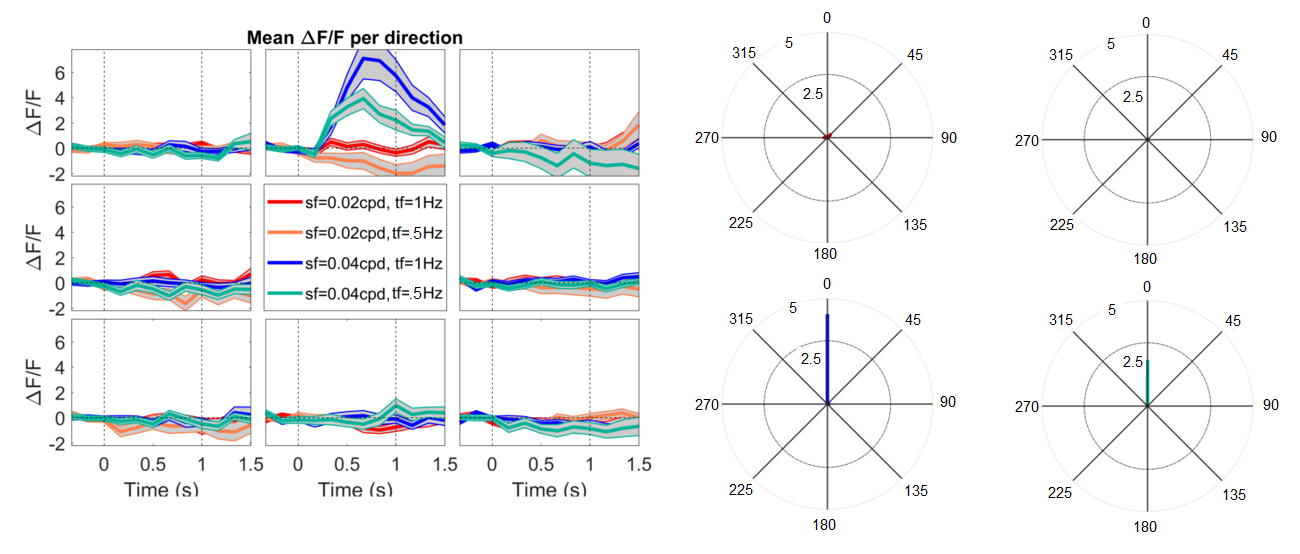
\includegraphics[width=12.5cm,height=12.5cm,keepaspectratio]{Figures/7.Results/tuning/CM006_pos1_p4_ROI0138.png} 
\caption{Tuning analysis for an example DS cell. Preferred $SF=0.04 cpd$, $TF=1 Hz$, temporal direction and horizontal orientation. DSI=0.393 ($p=6.05 \cdot 10^{-5}$), OSI=1 ($p=6.05 \cdot 10^{-5}$).}
\label{tuninganalysisDS}
\end{figure}

\section{SM analysis - individual cells}

SM analysis started with the mapping of responses during the protocol to corresponding stimuli types, from the 124 possible ones. During the experiments, 20 repetitions were held for most sessions. However, in the analysis, it was noticeable that responses [GET IMAGE] decreased a lot in the second part of the protocol, possibly due to anaesthesia cumulative effects and/or adaptation to the stimuli. Therefore, to prevent from adding noise to averaged measurements, the subsequent analysis was using only the 10 first repetitions of each trial type.

We start with individual cell example analysis, and present hereby two example cells' SM main effects.

\subsection{DS example cell}
\label{DSexamplecell}

We first consider, for simplification, a DS example cell: This cell only responds significantly to one of the four center directions used in this protocol.

Baseline-subtracted response strength for each trial by order of appearance can be plotted against time (stimulus onset at 0.5s), showing no visible structure (image \ref{individualDStrials}, left). 
Trials were then averaged by trial type and these were ordered in a given structure:

\begin{itemize}
\item \textbf{[1:4]} S1T, at the four directions (up, temporal, down, nasal); 
\item \textbf{[5:8]} C, analogous to above; 
\item \textbf{[9:12]} S1B, analogous to above;
\item \textbf{[13:16]} S1L, analogous to above;
\item \textbf{[17:20]} S1R, analogous to above; 
21:36 S1T+C, with first quarter (21:24) center up and surround in the 4 directions (up, temporal, down, nasal), second quarter (25:28) center temporal and surround in the 4 directions, third quarter (29:32) center down and surround in the 4 directions, and fourth quarter (33:36) center nasal and surround in the 4 directions;
\item \textbf{[37:52]} S1B+C, analogous to above;
\item \textbf{[53:68]} S1L+C, analogous to above;
\item \textbf{[69:84]} S1R+C, analogous to above;
\item \textbf{[85:100]} S2H+C, with first quarter (85:100) center up and the two horizontally positioned surrounds in the same of 4 directions (up, temporal, down, nasal), second quarter (89:92) center temporal and surrounds in the same of 4 directions, third quarter (93:96) center down and surrounds in the same of 4 directions, and fourth quarter (97:100) center nasal and surrounds in the the same of 4 directions;
\item \textbf{[101:104]} S2H, at the four directions (up, temporal, down, nasal);
\item \textbf{[105:120]} S2V+C, with first quarter (105:108) center up and the two vertically positioned surrounds in the same of 4 directions (up, temporal, down, nasal), second quarter (109:112) center temporal and surrounds in the same of 4 directions, third quarter (113:116) center down and surrounds in the same of 4 directions, and fourth quarter (117:120) center nasal and surrounds in the the same of 4 directions;
\item \textbf{[121:124]} S2V, at the four directions (up, temporal, down, nasal);
\end{itemize}

With this, when plotted per trial type average baseline-subtracted responses over repetitions as a function of time (figure \ref{individualDStrials}, right), we can denote that given sets of stimuli types evoke higher responses than others, with stronger spike responses being usually relative to the direction selective center-only response and to the four contiguous sets of the same center preferred direction with surround, as expected. Moreover, we also denote that responses are fixed to stimulus onset, validating appropriate synchronization in the experimental setup.

\begin{figure}[H] \centering 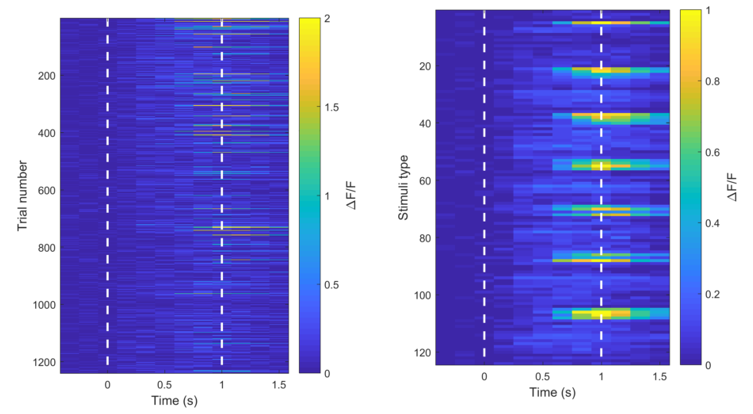
\includegraphics[width=14cm,height=14cm,keepaspectratio]{Figures/7.Results/individualSM/roi_29_mf379_pos5/roi29.png} 
\caption{SM protocol responses (dF/F) over time (s), for the example DS cell. Responses were baseline subtracted (0.5s) and stimulus onset centred at 0 s.
\newline \textbf{Left:} 1240 trial responses (10 repetitions, 124 trial types) as chronologically presented to the subjects, over the trial length. No structure is apparent.
\newline \textbf{Right:} Averaged repetition responses per trial type, ordered as determined on the text subsection \ref{DSexamplecell} over the trial length. Consistent structure is visible.}
\label{individualDStrials}
\end{figure}

Then we assess trial type responses within a given organization: First we show C stimuli responses, then S1 stimuli responses, and finally move to S1+C response profiles. We leave S2+C and S2 analysis for the population analysis section, focusing here on validating this protocol's analysis and interpreting the more simple found results in individual example cells.

In figure \ref{DSexamplecellcenter}, we observe that this cell portrays a large response to up center stimulation, but the responses for other directions are not substancial. This is a DS cell with up preferred direction. Figure \ref{DSexamplecellsurrounds} shows that surround-only stimulation did not hold any significant response for this cell, as required for this SM study.

\begin{figure}[H] \centering 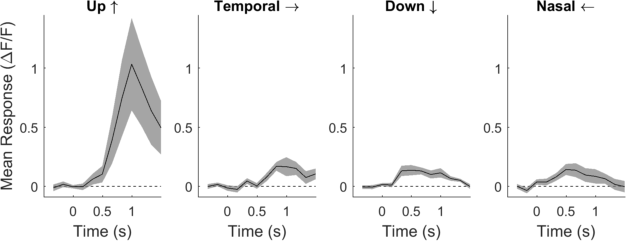
\includegraphics[width=11cm,height=11cm,keepaspectratio]{Figures/7.Results/individualSM/roi_29_mf379_pos5/1.png} 
\caption{Mean repetition trial response profiles for C conditions in the DS example cell, over trial time. The responses were baseline subtracted and the stimulus onset was centred at 0 s. Only the up center gratings direction evoked substantial significant responses.}
\label{DSexamplecellcenter}
\end{figure}

\begin{figure}[H] \centering 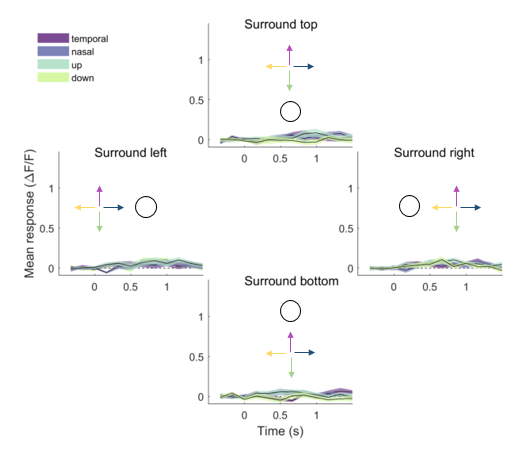
\includegraphics[width=10cm,height=10cm,keepaspectratio]{Figures/7.Results/individualSM/roi_29_mf379_pos5/2.png} 
\caption{Mean repetition trial response profiles for S1 conditions in the DS example cell, over trial time. The responses were baseline subtracted and the onset was at 0 s. No significant responses were present for this surround-only condition, as intended for SM analysis.
\label{DSexamplecellsurrounds}}
\end{figure}

In figure \ref{DSexamplecellSM} some SM results are shown. Only when center grating stimulation was on the up direction did any significant response hold (for simplicity not shown here, no responses were present either for horizontally or vertically positioned surrounds with non up-oriented center stimuli, supplementary figure \ref{s1}).

In this case, only surround suppression was present. Qualitatively, highest suppression is manifested for when surround stimulation is on the right, going in the down direction, followed by when it is also on the right, but going in the up direction and when it is going nasally in the top position.

\begin{figure}[H] \centering 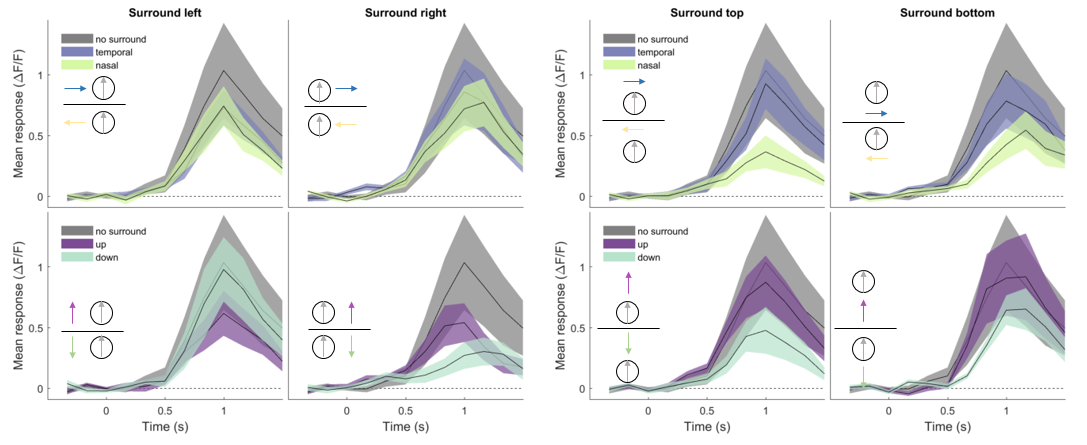
\includegraphics[width=15.9cm,height=15.9cm,keepaspectratio]{Figures/7.Results/individualSM/roi_29_mf379_pos5/3.png} 
\caption{S1+C effects for each center direction condition, averaged over 10 repetitions, over trial time, for the DS example cell. The responses were baseline subtracted and the onset was at 0 s. For comparisons, responses for center-only condition are represented as gray curves in each plot.
S1L+C, S1R+C, S1T+C and S1B+C respectively at each column, for up center condition. For each, surround gratings can be going temporally (blue curve), nasally (yellow curve), up (purple curve) or down (green curve).}
%S1L+C and S1R+C responses for center going temporally (left module), down (middle module) or nasally (right module). S1T+C and S1B+C responses are not shown here, as they portray similar non-responsive profiles.}
\label{DSexamplecellSM}
\end{figure}

Averaging the S1+C conditions over all of the center directions we find small responses and slight suppression average results (figure \ref{DSexamplecellaverage}), as these were diluted by the very little responses of this cell for other than up-directions. Suppression effects show the same qualitative results as above, but these were smaller than for the non-averaged center-up conditions; Over the population, facilitatory effects were rare, so this preliminary analysis did suggest (as realized with more examples and population analysis) that further analysis should be confined to the responsive center conditions, for minimizing noise additions to the results.

\begin{figure}[H] \centering 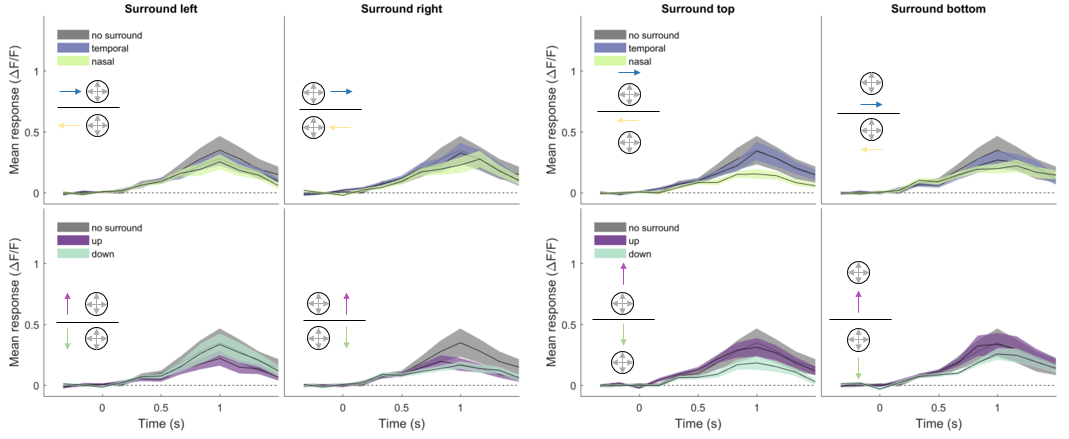
\includegraphics[width=15.9cm,height=15.9cm,keepaspectratio]{Figures/7.Results/individualSM/roi_29_mf379_pos5/4.png} 
\caption{Average responses for S1L+C, S1R+C, S1T+C and S1B+C, respectively from left to right. Conditions over all of the center directions.
\label{DSexamplecellaverage}}
\end{figure}

\subsection{OS example cell}

We present now the same sort of analysis for an OS example cell.

Again, in figure \ref{individualOStrials}, we see that plotting responses ordered chronologically does not show a response structure, but when these spikes are organized by stimulus type, here in the same number as explained in the above subsection, evident structure appears.

\begin{figure}[H] \centering 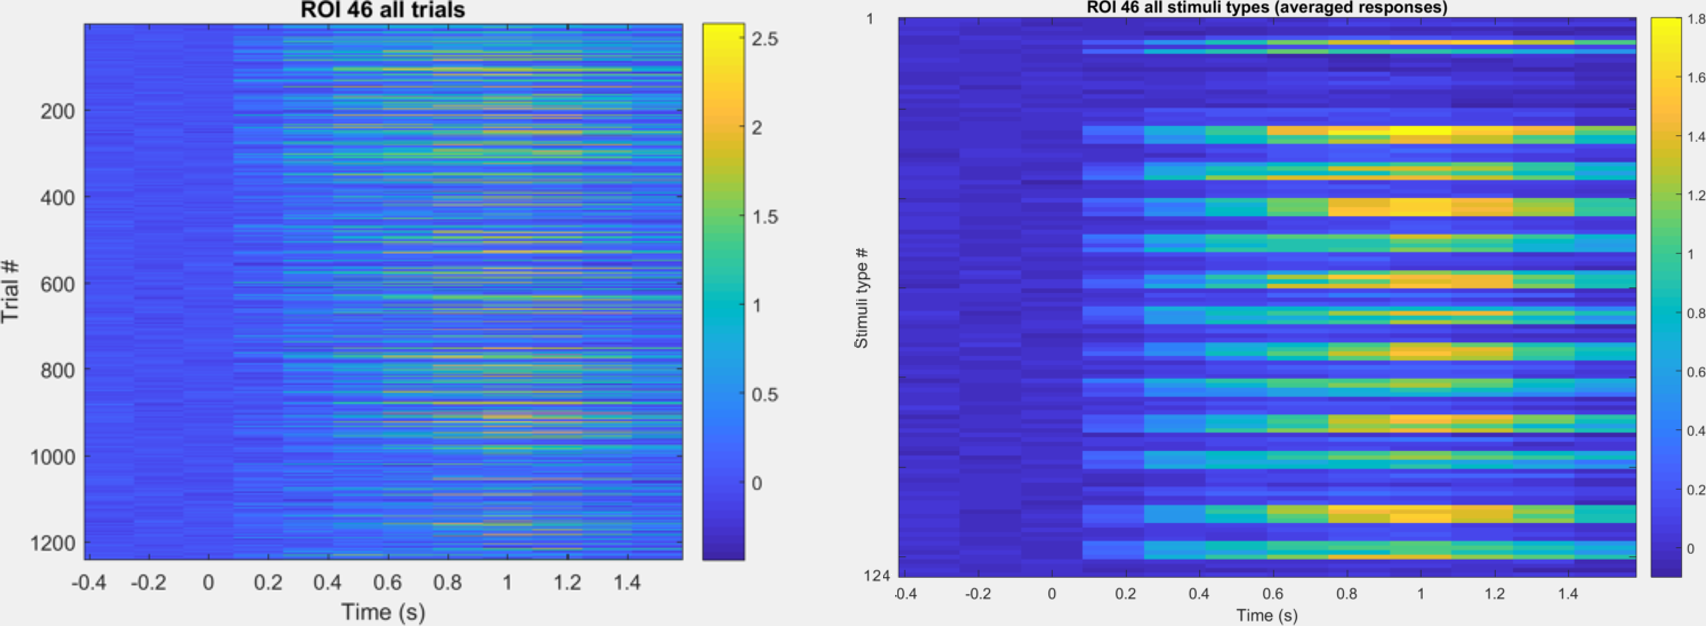
\includegraphics[width=14cm,height=14cm,keepaspectratio]{Figures/7.Results/individualSM/roi_46_mf379_pos2/roi46.png} 
\caption{SM protocol responses (dF/F) over time (s), for the example OS cell. The responses were baseline subtracted (0.5 s) and the stimulus onset was at 0 s.
\newline \textbf{Left:} 1240 trial responses (10 repetitions, 124 trial types) as chronologically presented to the subjects, over the trial length. No structure is apparent.
\newline \textbf{Right:} Averaged repetition responses per trial type, ordered as determined on the text subsection \ref{DSexamplecell} over the trial length. Consistent structure is visible. \label{individualOStrials}}
\end{figure}

We follow with the center only stimulation responses over the trial length (figure \ref{OSexamplecellcenter}). The cell is noticeably OS, with horizontal preferred orientation. As with the previous cell, no S1 condition held significant non-null responses, as intended for these SM analysis.

\begin{figure}[H] \centering 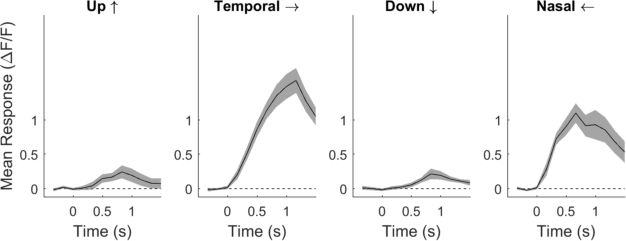
\includegraphics[width=11cm,height=11cm,keepaspectratio]{Figures/7.Results/individualSM/roi_46_mf379_pos2/1.png} 
\caption{Mean repetition trial response profiles for C conditions in the OS example cell, over trial time. The responses were baseline subtracted and the stimulus onset was centred at 0 s. The temporal and nasal center gratings directions evoked substantial significant responses, deeming the horizontal orientation the preferred orientation of this OS cell.}
\label{OSexamplecellcenter}
\end{figure}

In regards to the SM results, figure \ref{OSexamplecellSM} shows the most relevant profiles for this cell - for center going temporally or nasally. Other center direction conditions held no significant substantial  responses. 

In this case, the cell was barely suppressed by the surround, with the most noticeable effect being a facilitation one, for the center gratings going nasally, surround on top conditions, with surround going either nasally or temporally. As will be shown in the next section, these facilitatory effects were rare across the analysed population.

\begin{figure}[H] \centering 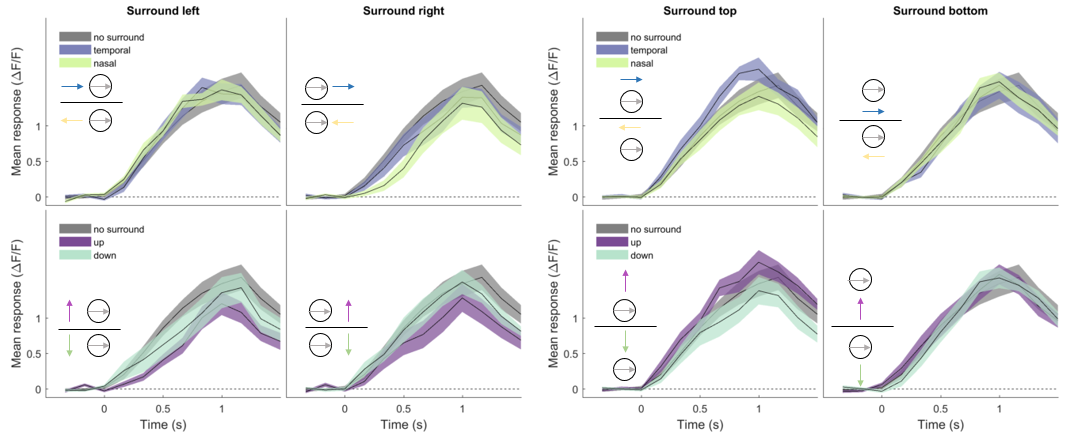
\includegraphics[width=15.9cm,height=15.9cm,keepaspectratio]{Figures/7.Results/individualSM/roi_46_mf379_pos2/3.png} 
\caption{S1+C effects for each center direction condition, averaged over 10 repetitions, over trial time, for the OS example cell. The responses were baseline subtracted and the onset was at 0 s. For comparisons, responses for center-only condition are represented as gray curves in each plot.
S1L+C, S1R+C, S1T+C and S1B+C respectively at each column, for temporal center condition. For each, surround gratings can be going temporally (blue curve), nasally (yellow curve), up (purple curve) or down (green curve).}
\label{OSexamplecellSM}
\end{figure}

\begin{figure}[H] \centering 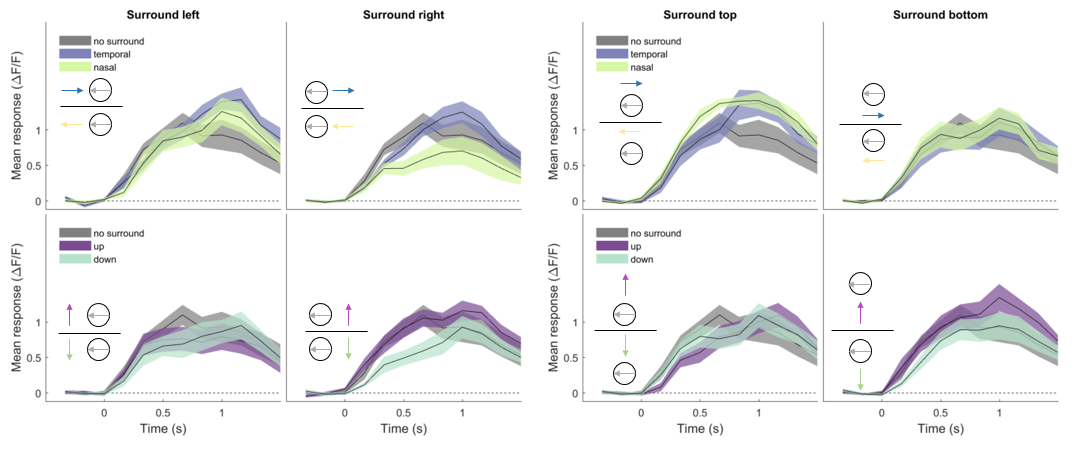
\includegraphics[width=15.9cm,height=15.9cm,keepaspectratio]{Figures/7.Results/individualSM/roi_46_mf379_pos2/4.png} 
\caption{S1+C effects for each center direction condition, averaged over 10 repetitions, over trial time, for the OS example cell. The responses were baseline subtracted and the onset was at 0 s. For comparisons, responses for center-only condition are represented as gray curves in each plot.
S1L+C, S1R+C, S1T+C and S1B+C respectively at each column, for nasal center condition. For each, surround gratings can be going temporally (blue curve), nasally (yellow curve), up (purple curve) or down (green curve).}
\label{OSexamplecellSM}
\end{figure}

\section{SM analysis - cells population}

After last section's scattered analysis, we follow with more general, systematic analysis, by investigating average effects on all of the cells population.

\subsection{Data ROI groups}

Firstly, we divide the available ROIs into different group classes.

In total, 2728 cells' trace responses were extracted from Suit2p pipeline (see section \ref{sec:Suit2ppipeline}).  From these, 2869 cells were responsive to some visual stimulation, as assessed with sign-tests over the differences between responses for stimulation and baseline times ($p<0.05$), for any of the trial types. Within these, 897 cells were significantly responsive to at least one of the center-only conditions (assessed with the same statistical test). This was the first condition for the cell to be SM analysed. These values are showed to scale on figure \ref{groups1}.

%\begin{figure}[H] \centering \includegraphics[width=5cm,height=5cm,keepaspectratio]{Figures/7.Results/data/ROIvisualCenter.png} 
%\caption{Scaled depiction of cell numbers for each responsiveness group condition: ROIs selected by Suit2p pipeline (blue), visually responsive ROIs (red) and center-only condition(s) responsive ROIs (green).}
%\label{groups1}
%\end{figure}

Within this last group of center-responsive ROIs, cells could also be divided in OS cells (n=472) and DS cells (n=371). Some DS cells were also OS cells (n=243). The remaining 600 cells were not found orientation selective. These assessments were made as described in subsection \ref{subsec:tuningresults}, but using the data set from the SM protocol's center only conditions. A scaled cell numbers diagram is presented in figure \ref{groups2}.
OS and DS cells were separately analysed in some relevant comparison cases in section \ref{sec:comparisons}.
%
%\begin{figure}[H] \centering 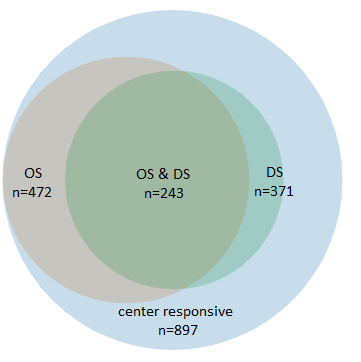
\includegraphics[width=5cm,height=5cm,keepaspectratio]{Figures/7.Results/data/centerOSDS.png} 
%\caption{Scaled depiction of cell numbers for each selectivity condition:Center responsive cells (blue), OS cells (red) and DS cells (green).}
%\label{groups2}
%\end{figure}

\begin{figure}[h]
    \centering
    \begin{minipage}[t]{.4\textwidth}
        \centering
\includegraphics[width=6cm,height=6cm,keepaspectratio]{Figures/7.Results/data/ROIvisualCenter.png} 
\caption{Scaled depiction of cell numbers for each responsiveness group condition: ROIs selected by Suit2p pipeline (blue), visually responsive ROIs (red) and center-only condition(s) responsive ROIs (green).\label{groups1}}
\end{minipage}\hspace{1cm}
\begin{minipage}[t]{0.4\textwidth}
\centering
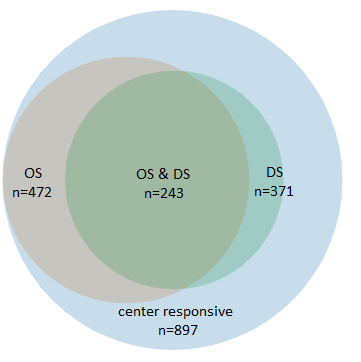
\includegraphics[width=6cm,height=6cm,keepaspectratio]{Figures/7.Results/data/centerOSDS.png} 
\caption{Scaled depiction of cell numbers for each selectivity condition: Center responsive cells (blue), OS cells (red) and DS cells (green).\label{groups2}}
\end{minipage}
\end{figure}

For all of the SM analysis, cells ought to be responsive to at least one of the center conditions, but were also conservatively required to hold no significant response for any of the relevant surround only conditions. In this way, we could be sure that independently of the receptive field measurements of each cell, the portrayed effects were in fact surround modulatory effects.
The majority (n=788) of the center responsive cells did not respond to any of the surrounds, showing that for these sessions the stimuli responses were well centred. For some of the analysis, we were able to loosen the requirements: There were 812 cells responding to the center and not to the horizontally positioned surrounds, while 864 cells responded to the center and not to the vertically positioned surrounds. These groups were again assessed with the same statistical sign-tests. These groups were used when analysis was projected in only one of the surround's position axis. Figure \ref{groups3} shows a cell numbers diagram for each of these conditions on the left, and the same simplified but scaled diagram on the right.

\begin{figure}[H] \centering 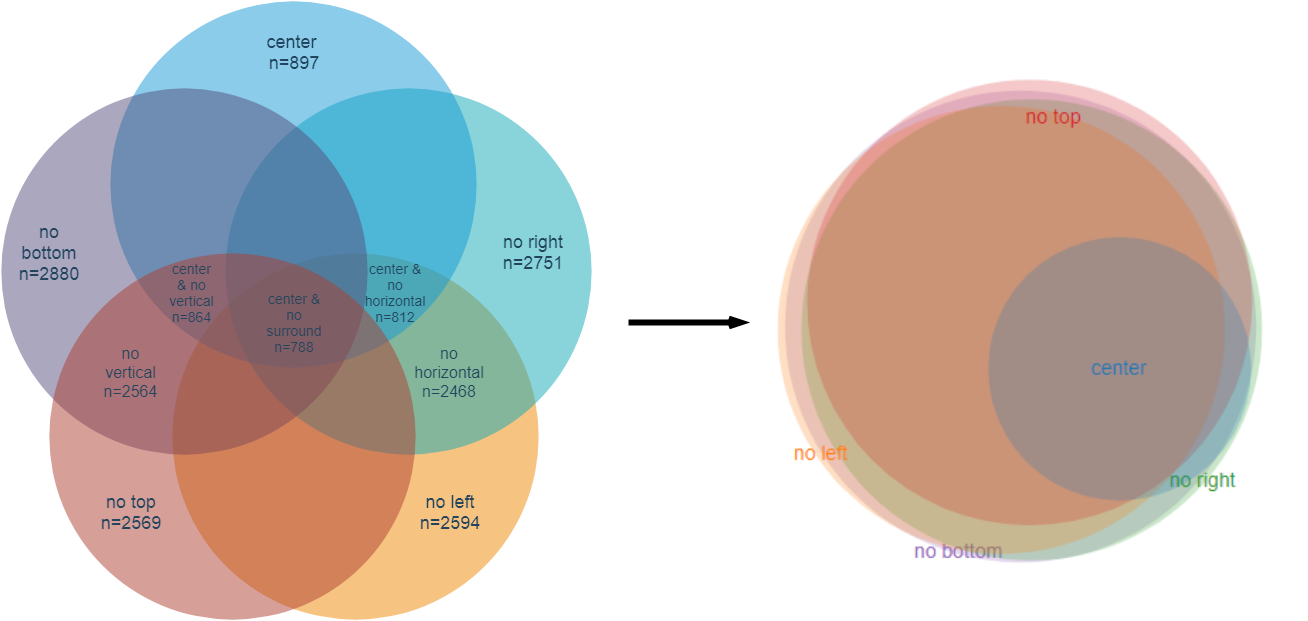
\includegraphics[width=15cm,height=15cm,keepaspectratio]{Figures/7.Results/data/SMdata.png} 
\caption{Diagram of cell numbers for each center and surround responsiveness condition, with detailed most relevant values (left) and scaled (right): Center responsive cells (blue), no S1L stimuli conditions responsive cells (yellow), no S1R stimuli conditions responsive cells (green), no S1T stimuli conditions responsive cells (red) and no S1B stimuli conditions responsive cells (green).}
\label{groups3}
\end{figure}

\subsection{RF center positions and SM protocol center-only: all population and per animal}

Beginning the following analysis, we first noticed that the dataset ROIS tended to become very weakly responsive for the second half of the SM protocol, possibly due to its extended length and anaesthesia condition. For this reason, all of the following analysis was done regarding only the 10 first trials of the SM protocol, for each trial type (1240 total stimuli). 


Starting with the population analysis, we first investigated the overall RF center locations of all the extracted ROIs, specifying also for the selected ROIs (center responsive and not surround only responsive). We found a consistent bias in our data set for ROIs with higher elevation RF centres, for both the cases of all of the ROIs and the case of the selected ROIs (\ref{allRF}).  The same bias was found when separating the ROIs per animal and per session (for an example, \ref{exRF}). For this reason, subsequent analysis was not conducted for comparing top and bottom conditions, nor for comparing horizontally-positioned with vertically-positioned surround conditions.

\begin{figure}[h]
    \centering
    \begin{minipage}[t]{.4\textwidth}
        \centering 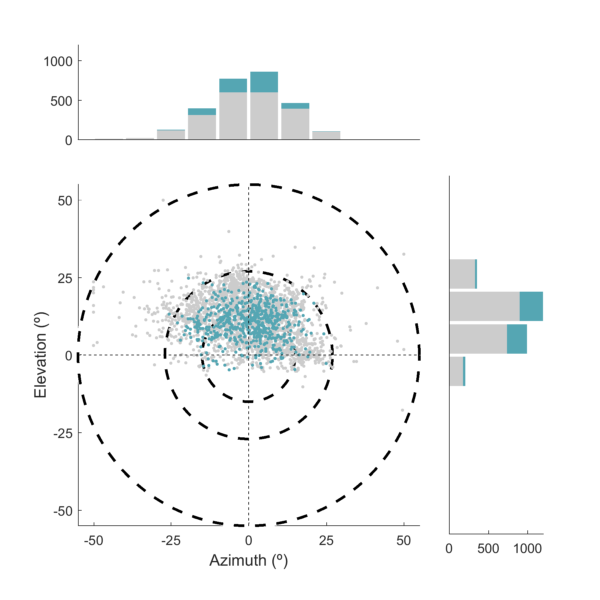
\includegraphics[width=7.8cm,height=7.8cm,keepaspectratio]{Figures/7.Results/finalPopulation/sel/popPlots_rfPositions_allSessions.png} 
\caption{RF center coordinates for all the ROIs (gray, n=3728), specifying the selected center responsive and not surround only responsive ROIs (turquoise, n=788). Dashed lines represent the stimuli sizes: inner circle for the center stimuli, outer annulus for the different surround positions. Frequency histograms for both elevation (side) and azimuth (top) locations.}
\label{allRF}
\end{minipage}\hspace{1cm}
\begin{minipage}[t]{.4\textwidth}
\centering 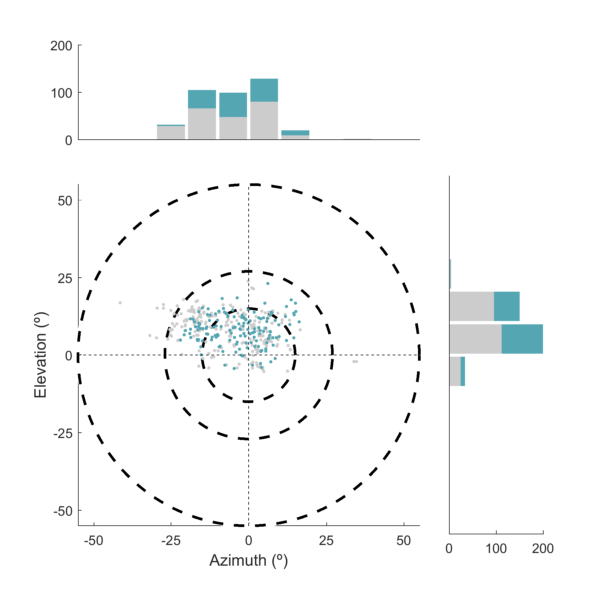
\includegraphics[width=7.8cm,height=7.8cm,keepaspectratio]{Figures/7.Results/finalPopulation/sel/popPlots_RFpos_Animal4_Session5.png} 
\caption{RF center coordinates for the ROIs from an example animal and session (gray, n=236), specifying the selected center responsive and not surround only responsive ROIs (turquoise, n=153).} 
\label{exRF}
\end{minipage}
\end{figure}
%\begin{figure}[H] \centering 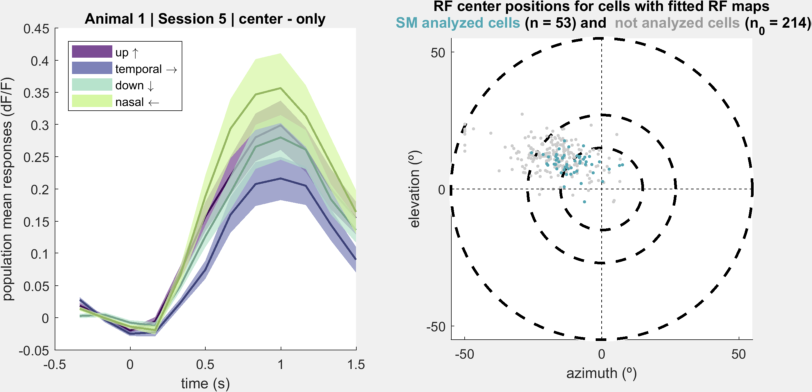
\includegraphics[width=12cm,height=12cm,keepaspectratio]{Figures/7.Results/population/sel/2_popPlots_Animal1_Session5.png} 
%%\caption{2 popPlots Animal1 Session5.} 
%\end{figure}

%\begin{figure}[H] \centering 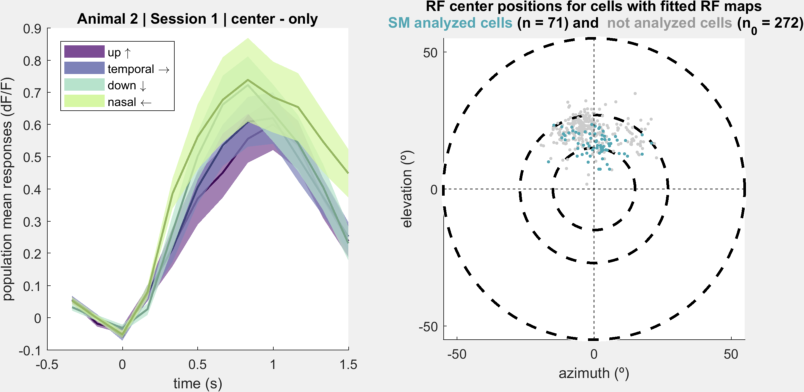
\includegraphics[width=12cm,height=12cm,keepaspectratio]{Figures/7.Results/population/sel/3_popPlots_Animal2_Session1.png} 
%%\caption{3 popPlots Animal2 Session1.} 
%\end{figure}
%
%\begin{figure}[H] \centering 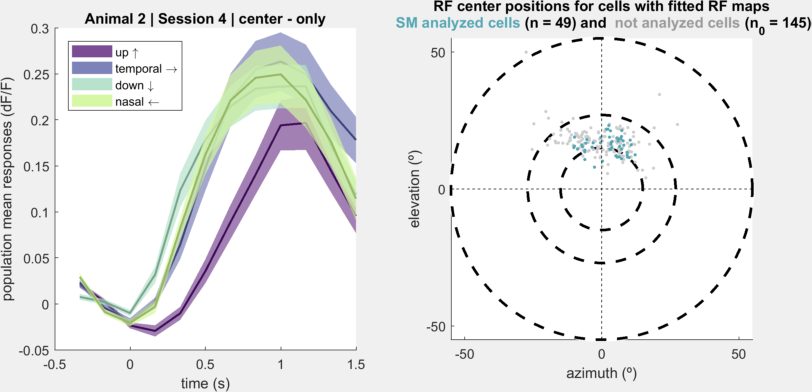
\includegraphics[width=13cm,height=13cm,keepaspectratio]{Figures/7.Results/population/sel/4_popPlots_Animal2_Session4.png} 
%%\caption{4 popPlots Animal2 Session4} 
%\end{figure}
%
%\begin{figure}[H] \centering 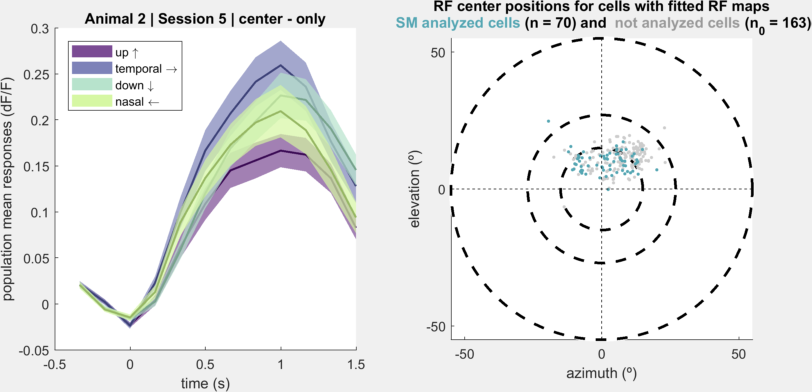
\includegraphics[width=13cm,height=13cm,keepaspectratio]{Figures/7.Results/population/sel/5_popPlots_Animal2_Session5.png} 
%%\caption{5_popPlots_Animal2_Session5} 
%\end{figure}



%\begin{figure}[H] \centering 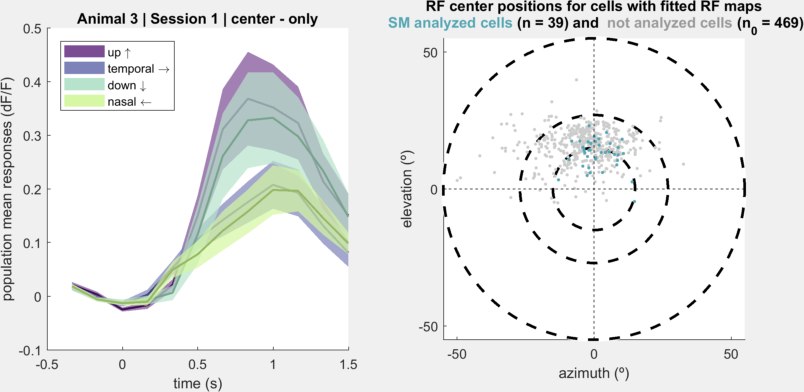
\includegraphics[width=13cm,height=13cm,keepaspectratio]{Figures/7.Results/population/sel/7_popPlots_Animal3_Session1.png} 
%%\caption{7_popPlots_Animal3_Session1} 
%\end{figure}
%
%\begin{figure}[H] \centering 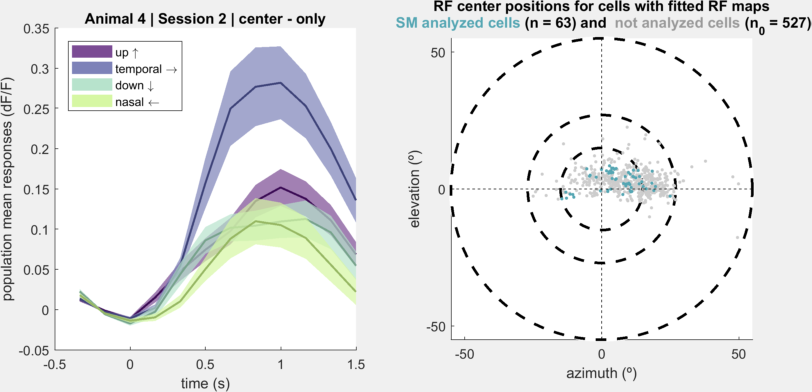
\includegraphics[width=13cm,height=13cm,keepaspectratio]{Figures/7.Results/population/sel/8_popPlots_Animal4_Session2.png} 
%%\caption{8_popPlots_Animal4_Session2} 
%\end{figure}
%
%\begin{figure}[H] \centering 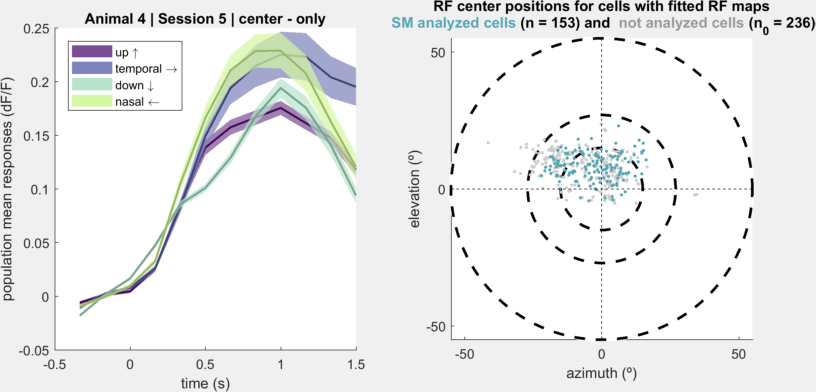
\includegraphics[width=13cm,height=13cm,keepaspectratio]{Figures/7.Results/population/sel/9_popPlots_Animal4_Session5.png} 
%%\caption{9_popPlots_Animal4_Session5} 
%\end{figure}

Next, we assess the selected ROIs responses to the center only conditions (for the four cardinal directions). For this, we separate the cell's by their orientation selectivity. Non-OS cells have distributed responses across the four directions (figure \ref{nonOS}). We are also able to observe that different neurons respond at different times, in relation to the stimulus onset.

\begin{figure}[H] \centering 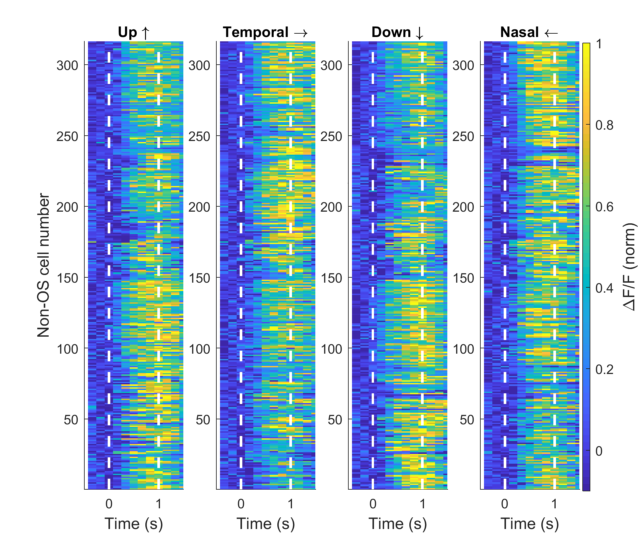
\includegraphics[width=12cm,height=12cm,keepaspectratio]{Figures/7.Results/finalPopulation/sel/popPlots_nonOS_centerOnly.png} 
\caption{Normalized responses across non-OS neurons, for the C conditions, each panel respectively for on of the four directions up, temporal, down and nasal. Responses are computed as the mean of the trial repetitions (10) for that cell and that stimulus condition. Dashed lines mark stimulus onset and offset.} 
\label{nonOS}
\end{figure}

We then do the same verifications, for OS selected cells: OS neurons with horizontal preferred orientation and  OS (figure \ref{OShorz}) neurons with vertical preferred orientation (figure \ref{OSvert}). Indeed, we find that horizontal OS cells respond more for temporal and nasal moving center gratings, while vertical OS cells respond for up and down moving center gratings.
\vspace*{-0.4cm}
\begin{figure}[H] \centering 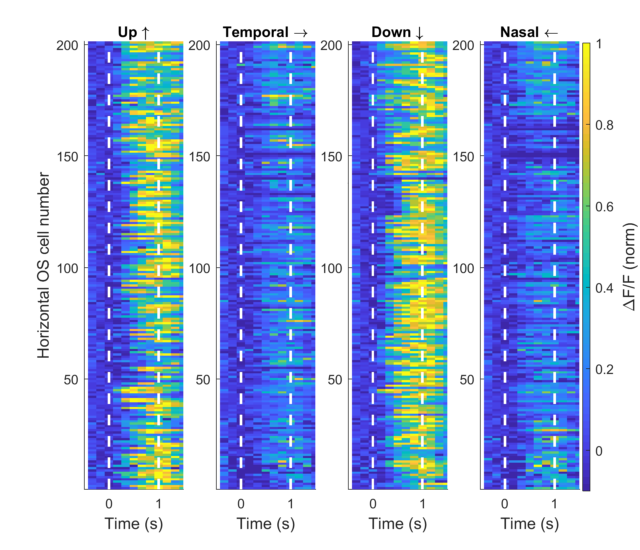
\includegraphics[width=11cm,height=11cm,keepaspectratio]{Figures/7.Results/finalPopulation/sel/popPlots_horzOS_centerOnly.png} 
\vspace*{-0.2cm}\caption{Normalized responses across horizontal OS neurons, for the C conditions, each panel respectively for one of the four directions up, temporal, down and nasal. Responses are computed as the mean of the trial repetitions (10) for that cell and that stimulus condition. Dashed lines mark stimulus onset and offset.} \label{OShorz}
\end{figure}
\vspace*{-0.4cm}
\begin{figure}[H] \centering 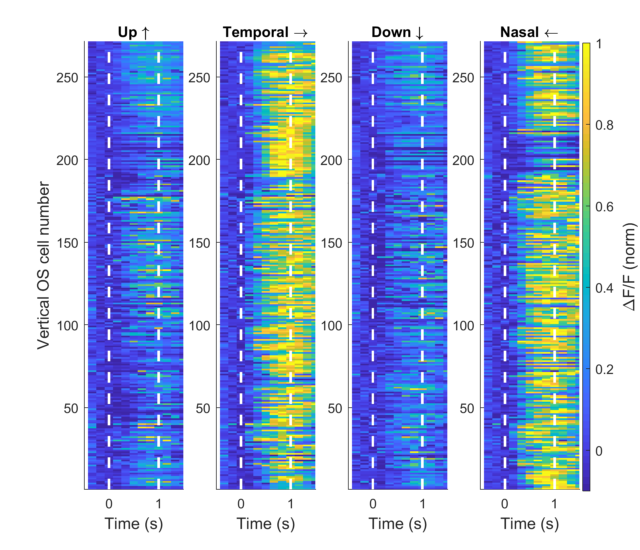
\includegraphics[width=11cm,height=11cm,keepaspectratio]{Figures/7.Results/finalPopulation/sel/popPlots_vertOS_centerOnly.png} 
\vspace*{-0.2cm}\caption{Normalized responses across vertical OS neurons, for the C conditions, each panel respectively for one of the four directions up, temporal, down and nasal. Responses are computed as the mean of the trial repetitions (10) for that cell and that stimulus condition. Dashed lines mark stimulus onset and offset.} \label{OSvert}
\end{figure}

\subsection{Comparisons between conditions}
\label{sec:comparisons}

At this point, the analysis continues with comparisons between multiple S1+C and S2+C surround and center configurations, to investigate the existence of biases or trends regarding the surround positions, orientations, directions, center orientation, direction, OS and/or DS preferences, as well as combinations of these factors. Each comparison was thus done with different numbers of cells and different stimuli numbers of conditions. 

For each of these comparisons, the intended outputs are both the effect's strength and statistical significance. 

\begin{enumerate}
\item First, we regard how differently does the population respond to the center-only C condition and the first of the pooled configuration sets to compare, within a scatter-plot (top, first panel of image \ref{1}). 

\item Second, we regard the same for the other pooled configuration set to compare (top, second of image \ref{1}). 

\item The population averaged (across ROIs, pooled conditions and trial repetitions) response trace is also extracted for each of these configuration sets and compared with the population averaged (across ROIs and trial repetitions) appropriate center-only condition response trace (top third panel of image \ref{1}, first panel of all subsequent comparison figures).

\item Next, we compare the responses between the two configuration sets, within a scatter plot (bottom first panel of image \ref{1}).

\item Then, we compare the SM indexes ($SMI$) of the pooled ROIs - a measurement of the surround modulatory effect strenght-, in a scatter-plot, for each configuration set (bottom, second panel of image \ref{1}; second panel of the other comparison images). For every stimuli surround-center condition, one can compute:

\begin{equation}
SMI_a=\dfrac{\bar{R_{a}}-\bar{R_C}}{\bar{R_a}+\bar{R_C}}
\end{equation}

With $\bar{R_a}$ the average (across trial repetitions and stimulus time) surround and center condition at hand, and $\bar{R_C}$ the average  (across trial repetitions and stimulus time) of the respective center-only condition.

The cell's $SMI$ to consider for a given set of configurations then averages across the $SMI_a$s for each of the pooled conditions.

A method to regard the effects tendencies and significance, involves single-neuron analysis: assessing how many neurons respond significantly to one or to the other set of configurations being compared, with a rank-sum test, at p-value threshold $p=0.05$. These are presented in the scatter-plot of each figure, respectively coloured, along with its counts. 

\item Finally, we plot the frequency histogram of the difference between the compared SM effects for one and the other configuration sets, within the population,$\Delta SMI$ (last panels of image \ref{1} and all following comparison figures). We additionally calculate the average of these $\Delta SMI$, $\mu$ and the correspondent p-value, calculated with a sign-test. This measures SM asymmetry between the two configuration sets and correspondent significance.

\end{enumerate}

At the side of each comparison figure, there's a diagram of the pooled stimuli conditions for each configuration set (blue and red). We enhance the frame for configuration sets towards which the computed $\mu$ tend to - that is, the configuration set for with the population tends to entail higher suppression, on average - when the obtained p-value is less than $0.05$. This expresses SM tendencies towards one or the other configuration set.

However, in a more statistically conservative approach, considering the multi-inference nature of this study, the Holm-Bonferroni method was used to compensate the multiple comparisons problem (see in the statistical tools chapter, \ref{sec:StatisticalTests}), delivering a powerful way of assessing each comparison's significance. The p-value family threshold was $\alpha=0.05$. If a test was accepted, with the Bonferroni correction, an asterisk is also drawn in the last panel of the respective comparison figure to express statistical significance.

\subsubsection{Surround number effect}

We start with the surround number effect: We find a large and significant differential effect of higher suppression for double surround conditions over one surround condition. Moreover, suppression was also notable, for all of the conditions, in particular for the 2S+C pooled conditions.

\begin{figure}[H] \centering 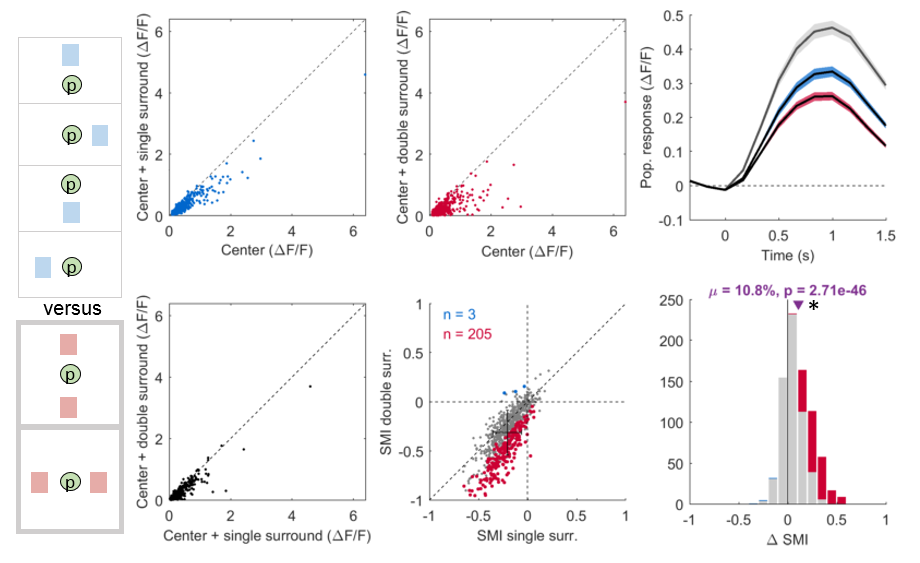
\includegraphics[width=12cm,height=12cm,keepaspectratio]{Figures/7.Results/finalPopulation/sel/diagrams/1.png} 
\caption{Surround number effect: Single surround versus double surround, with center gratings moving in the most responsive direction; $n=788$, 16 (single) and 8 (double) pooled conditions per configuration set.} 
\end{figure}

Across comparisons, we consistently found that two surround conditions held the most differentiated effects. This was a noted result, and thus we next perform the comparisons, when possible, with the 2S+C stimuli sets.

We disregard the intermediate panels in the next comparison plots. 

\subsubsection{Surround-RF distance effect and Surround position effect}

%\begin{figure}[H] \centering 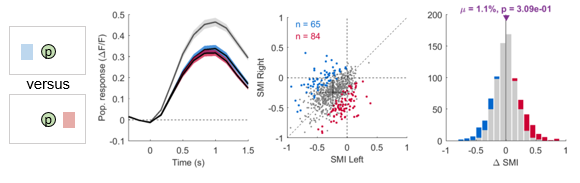
\includegraphics[width=11cm,height=11cm,keepaspectratio]{Figures/7.Results/finalPopulation/sel/diagrams/2.png} 
%%\caption{13_popPlots_VisROIs_CprefDir_Snumber} 
%\end{figure}


%\begin{figure}[H] \centering 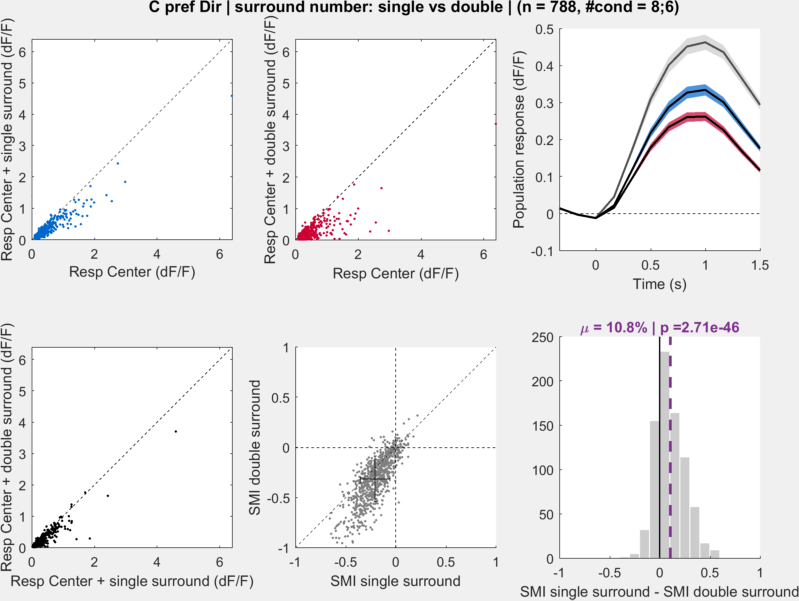
\includegraphics[width=12cm,height=12cm,keepaspectratio]{Figures/7.Results/finalPopulation/sel/13_popPlots_VisROIs_CprefDir_Snumber.png} 
%%\caption{13_popPlots_VisROIs_CprefDir_Snumber} 
%\end{figure}
%
%\begin{figure}[H] \centering 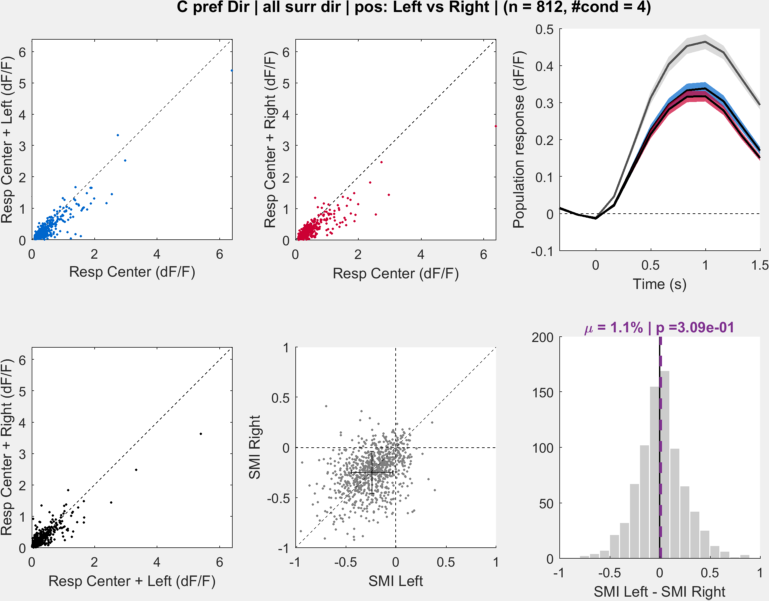
\includegraphics[width=12cm,height=12cm,keepaspectratio]{Figures/7.Results/finalPopulation/sel/14_popPlots_VisROIs_CprefDir_SposLeftRight.png} 
%%\caption{14_popPlots_VisROIs_CprefDir_SposLeftRight} 
%\end{figure}

Comparing the left versus right surround conditions, we first assessed the relationship between the SMI and the RF azimuth center position. We found, with a multiple regression, that, for both left and right cases, the SMI depended linearly on the azimuth RF center coordinate (p=0.002 and p=0.0056, respectively - figure \ref{reg}.

We then wanted to find if this effect differed between the left and the right surround cases. For this, we held a double permutation test with 10000 resamples, for both the slope and the offset of the regression for SMI_{Left} and for SMI_{Right}, and tested the null hypothesis that the new resamples, the same ROIs, but randomly attributed to either SMI_{Left} regression or SMI_{Right} regression, did not differ from the original distribution of ROI points. We obtained for the offset $p=0.1472$ and for the slope $p=0.8712$. This means that we cannot reject the null hypothesis, so the differences between left and right cases regression slopes and offsets are thus regarded as non significant. This finding suggests a distance effect: The SMI becomes increasingly stronger, the closer the RF center is to it, even though, we note again, the surround-only condition does not evoke any response. 

\begin{figure}[H] \centering 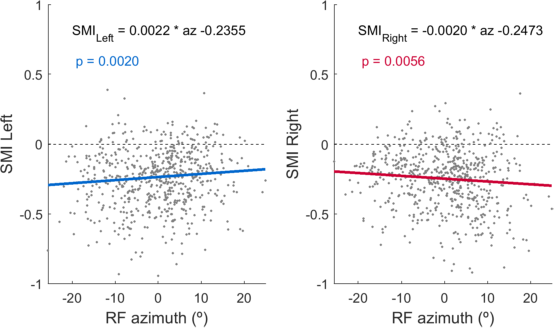
\includegraphics[width=10cm,height=10cm,keepaspectratio]{Figures/7.Results/finalPopulation/sel/reg.png} 
\caption{SMI of the selected ROIs, across S1L+C conditions (left panel) and S1R+C conditions (right panel), as a function of azimuth RF center coordinate. Superimposed multiple regression line, equation and p-value.} \label{reg}
\end{figure}

Finding this distance effect, we then chose a balanced dataset across azimuth, and compared the left and right surround modulatory effects (figure \ref{2}). A tendency seemed to appear for left surround suppressing more than right surround, but this result held no significance.

\begin{figure}[H] \centering 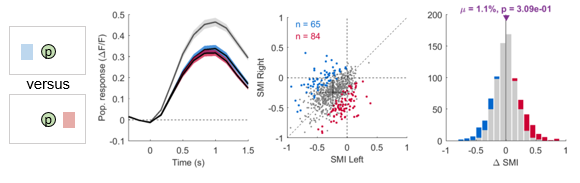
\includegraphics[width=12cm,height=12cm,keepaspectratio]{Figures/7.Results/finalPopulation/sel/diagrams/2.png} 
\caption{Position effect: left versus right surround, with center moving in the most responsive direction; Balanced dataset over RF azimuth location; $n=434$, 4 pooled conditions per configuration set.} \label{2}
\end{figure}

\subsubsection{Surround direction effect}

To determine the surround direction effect, we started by comparing the up versus down conditions (figure \ref{3}, double surround; Weaker qualitative result with the same tendency for one surround, as was the case in all following comparisons). We found no differential effect and high consistent suppression.

\begin{figure}[H] \centering 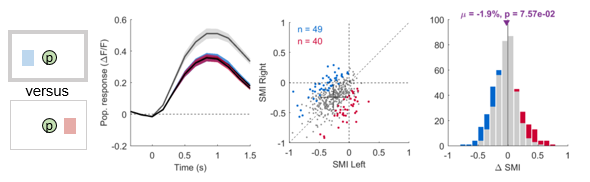
\includegraphics[width=12cm,height=12cm,keepaspectratio]{Figures/7.Results/finalPopulation/sel/diagrams/3.png} 
\caption{Direction effect: up versus down surround, with center moving in the most responsive direction and double surround conditions;  $n=788$, 2 pooled conditions per configuration set.}
\label{3} 
\end{figure}

For temporal versus nasal conditions (figure \ref{4}), the differential effect tended to increase, with higher suppression for nasally moving stimuli. However, correcting for multiple inferences, the result was not found significant.

\begin{figure}[H] \centering 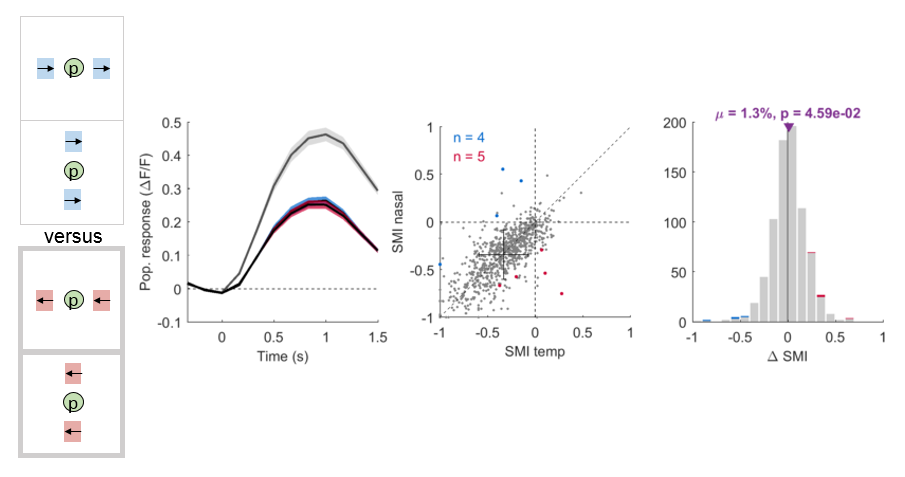
\includegraphics[width=12cm,height=12cm,keepaspectratio]{Figures/7.Results/finalPopulation/sel/diagrams/4.png} 
\caption{Direction effect: temporal versus nasal surround, with center moving in the most responsive direction and double surround conditions;  $n=788$, 2 pooled conditions per configuration set.} 
\label{4}
\end{figure}

\subsubsection{Surround orientation effect}

We follow with the orientation effect (figure \ref{5} A tendency appeared for higher suppression when surround stimuli moving horizontally versus moving vertically. However, corrected with Bonferroni method, this result did not hold significant.

\begin{figure}[H] \centering 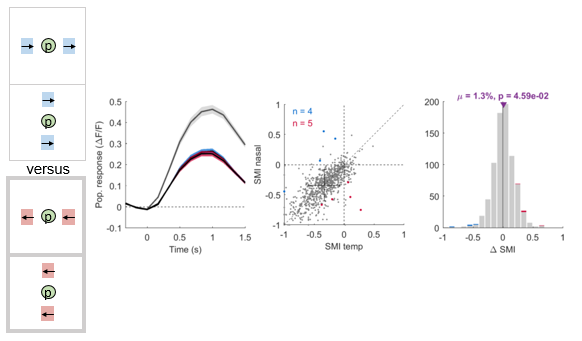
\includegraphics[width=12cm,height=12cm,keepaspectratio]{Figures/7.Results/finalPopulation/sel/diagrams/5.png} 
\caption{Orientation effect: horizontal versus vertical surround, with center moving in the most responsive direction and double surround conditions;  $n=788$, 4 pooled conditions per configuration set.} 
\label{5}
\end{figure}

\subsubsection{Surround orientation alignment effect (position and orientation)}

Combining position and orientation surround effects, we regard the surround orientation alignment effect of stimuli in the colinear versus the flanking alignments (figure \ref{6}). We found a substantial and significant difference between the pooled configuration sets: colinearity suppressed to a significantly higher degree than flanking conditions.

\begin{figure}[H] \centering 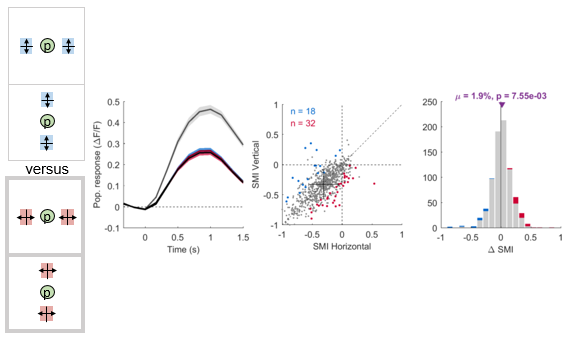
\includegraphics[width=12cm,height=12cm,keepaspectratio]{Figures/7.Results/finalPopulation/sel/diagrams/6.png} 
\caption{Alignment effect: colinear versus flanking surround, with center moving in the most responsive direction and double surround conditions;  $n=788$, 4 pooled conditions per configuration set.} 
\label{6}
\end{figure}

\subsubsection{Center and surround relative orientation effect, with center OS preference}

Now regarding as well the center gratings orientation of movement, relative to the surround's, we assess the Center-surround relative orientation effect (figure \ref{7}). A significant large result is observed: Iso-oriented surround suppresses tendentiously more than cross-oriented surround gratings.

\begin{figure}[H] \centering 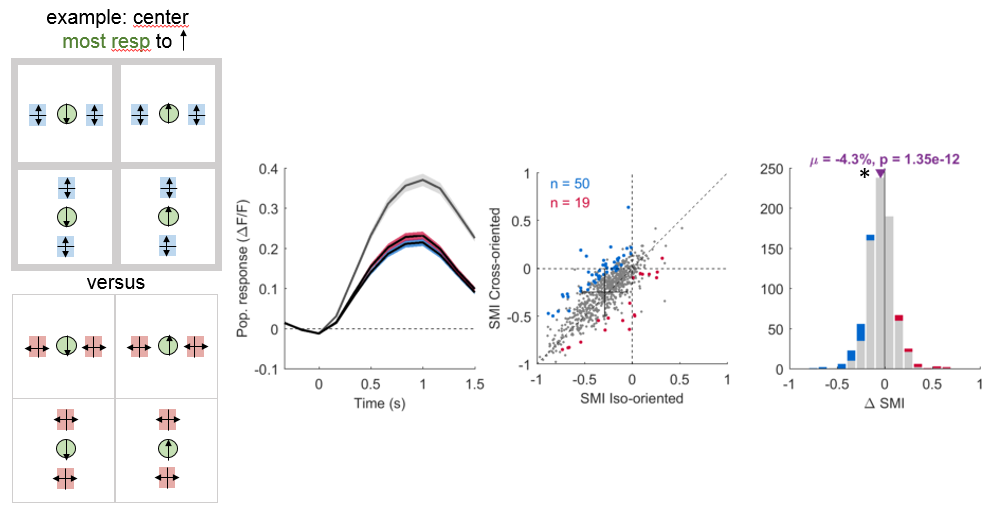
\includegraphics[width=12cm,height=12cm,keepaspectratio]{Figures/7.Results/finalPopulation/sel/diagrams/7.png} 
\caption{Relative orientation effect: iso-oriented versus cross-oriented surround, with center moving in the most responsive direction and double surround conditions;  $n=788$, 8 pooled conditions per configuration set.} 
\label{7}
\end{figure}

We also check this comparison for OS only cells, first when the center is in the preferred orientation (image \ref{8}). The same qualitative result holds significant, however less strong than in the non-OS case.

\begin{figure}[H] \centering 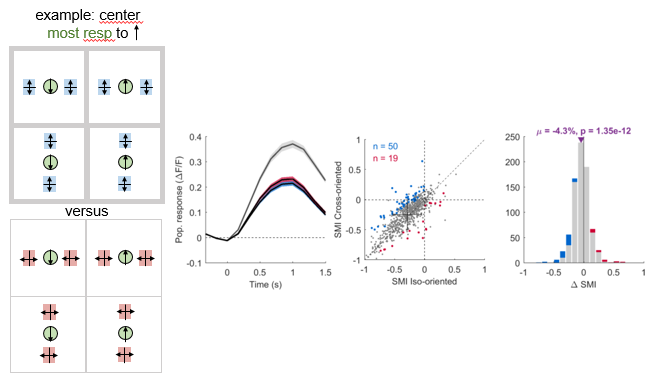
\includegraphics[width=12cm,height=12cm,keepaspectratio]{Figures/7.Results/finalPopulation/sel/diagrams/8.png} 
\caption{Relative orientation effect: iso-oriented versus cross-oriented surround, OS ROIs with center in the preferred orientation and double surround conditions;  $n=472$, 8 pooled conditions per configuration set.} \label{8}
\end{figure}

The same comparison is then performed for OS only cells, when the center is in the anti-preferred orientation (image \ref{9}). The same tendency as in the previous cases is apparent, but significance is lost. In fact, this condition has much fewer available ROIs ($n=68$) since for this analysis the neurons must be OS for one orientation, but still respond to the other to be chosen, which is more stringent than for previous ROI sets.

\begin{figure}[H] \centering 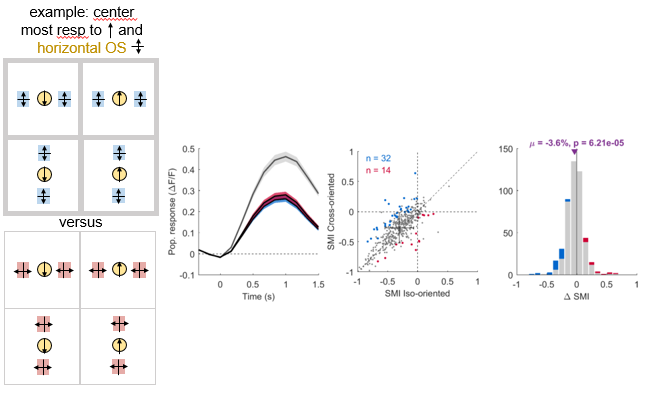
\includegraphics[width=12cm,height=12cm,keepaspectratio]{Figures/7.Results/finalPopulation/sel/diagrams/9.png} 
\caption{Relative orientation effect: iso-oriented versus cross-oriented surround, OS ROIs with center in the anti-preferred orientation and double surround conditions;  $n=68$, 8 pooled conditions per configuration set.} \label{9} 
\end{figure}

\subsubsection{Interactions between surround orientation alignment and surround-center relative orientation effects}

We now pool different conditions within the orientation alignment and the relative orientation effects, to investigate interaction effects between these two factors.

First, we take

\begin{figure}[H] \centering 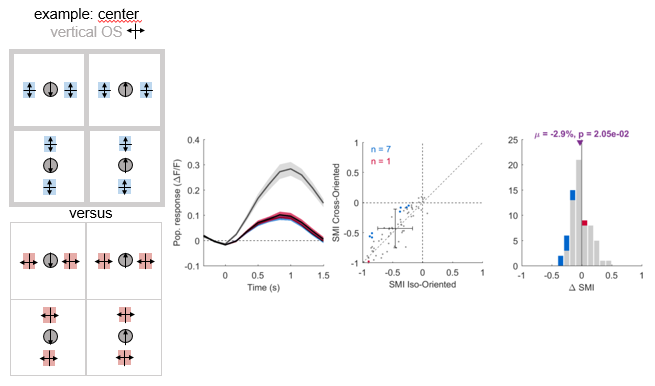
\includegraphics[width=12cm,height=12cm,keepaspectratio]{Figures/7.Results/finalPopulation/sel/diagrams/10.png} 
%\caption{13_popPlots_VisROIs_CprefDir_Snumber} 
\end{figure}

\begin{figure}[H] \centering 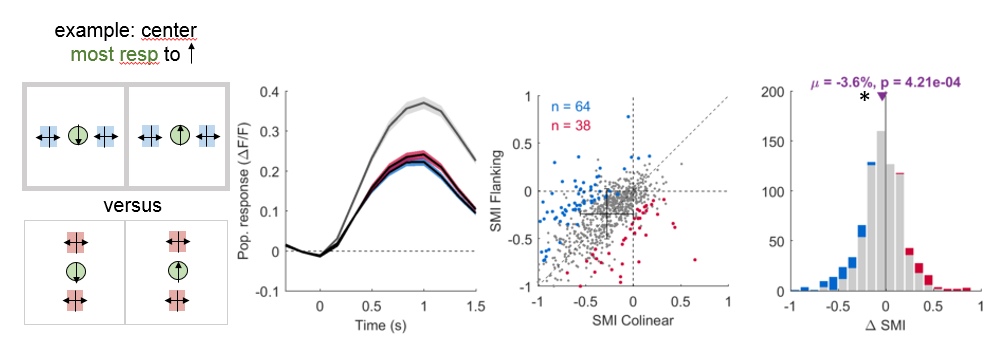
\includegraphics[width=12cm,height=12cm,keepaspectratio]{Figures/7.Results/finalPopulation/sel/diagrams/11.png} 
%\caption{13_popPlots_VisROIs_CprefDir_Snumber} 
\end{figure}

\begin{figure}[H] \centering 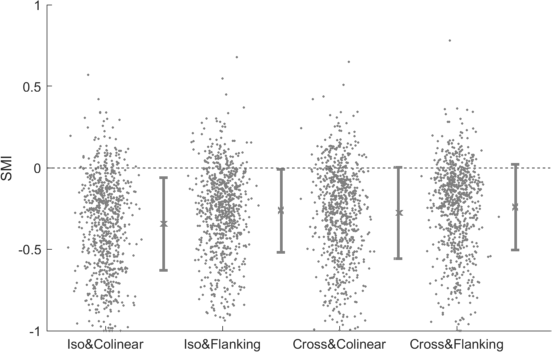
\includegraphics[width=12cm,height=12cm,keepaspectratio]{Figures/7.Results/finalPopulation/sel/popPlots_VisROIs_Cor_2SalignmentAngle.png} 
%\caption{26_popPlots_VisROIs_Cor_2SalignmentAngle} 
\end{figure}

%\begin{table}[H]
%\begin{center}\par
%\scalebox{0.85}{
%\begin{tabular}{c|cccccccccccccccccccccccccc}
%\hline 
% 
%    
%\multicolumn{1}{c}{Feature} & Value \\
%           
%           \hline
%           \hline
%
%\multicolumn{1}{c}{stimulus size (º)} & 30 \\
%\multicolumn{1}{c}{stimulus center (º)} & [0, 0] \\
%\multicolumn{1}{c}{stim directions (º)} & [0 45 90 135 180 225 270 315] \\
%\multicolumn{1}{c}{spatial frequency (/º)} & [0.02 0.04] \\
%\multicolumn{1}{c}{temporal frequency (Hz)}& [0.5 1] \\
%\multicolumn{1}{c}{dark, stim, background light} & [0 204 102] \\
%\hline
%        
%\end{tabular}}
% \caption{Configurations regarding the tuning mapping protocol stimuli properties.}
%    \vspace{-5mm}
%    \label{table:tuning}
%\end{center}
%\end{table}

\subsubsection{Interactions between surround orientation alignment, surround-center relative orientation effects and center OS preference}

\begin{figure}[H] \centering 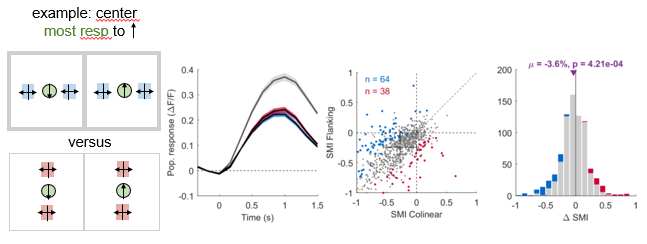
\includegraphics[width=12cm,height=12cm,keepaspectratio]{Figures/7.Results/finalPopulation/sel/diagrams/12.png} 
%\caption{13_popPlots_VisROIs_CprefDir_Snumber} 
\end{figure}

\begin{figure}[H] \centering 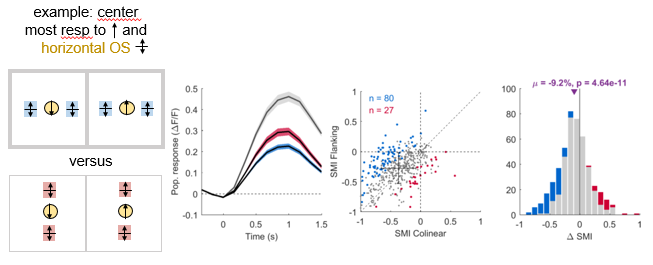
\includegraphics[width=12cm,height=12cm,keepaspectratio]{Figures/7.Results/finalPopulation/sel/diagrams/13.png} 
%\caption{13_popPlots_VisROIs_CprefDir_Snumber} 
\end{figure}

\begin{figure}[H] \centering 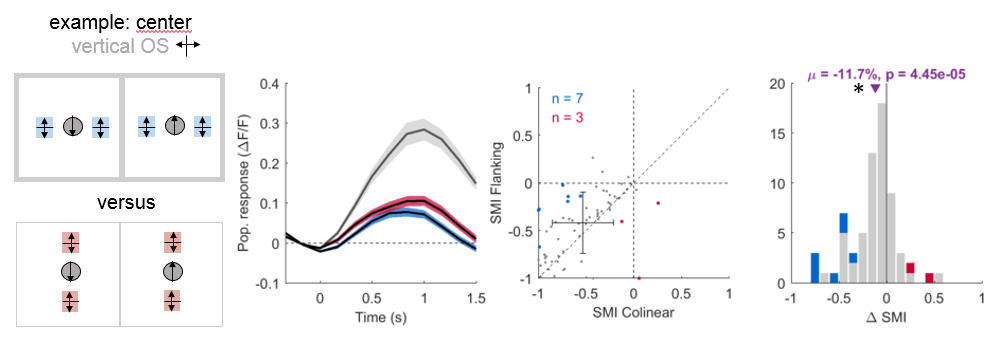
\includegraphics[width=12cm,height=12cm,keepaspectratio]{Figures/7.Results/finalPopulation/sel/diagrams/14.png} 
%\caption{13_popPlots_VisROIs_CprefDir_Snumber} 
\end{figure}

\begin{figure}[H] \centering 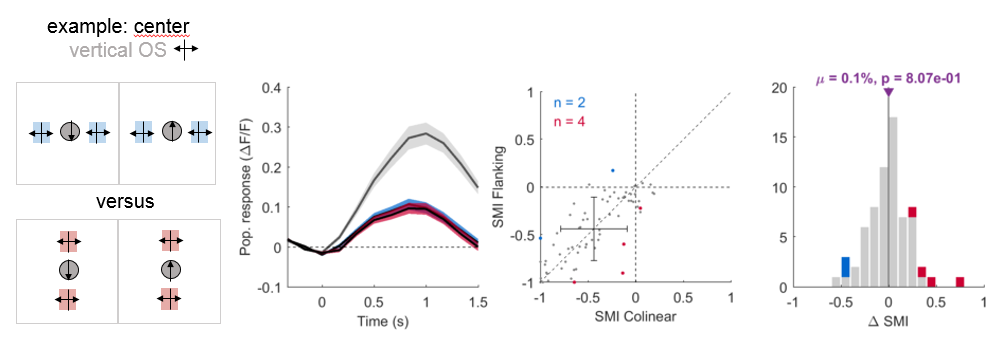
\includegraphics[width=12cm,height=12cm,keepaspectratio]{Figures/7.Results/finalPopulation/sel/diagrams/15.png} 
%\caption{13_popPlots_VisROIs_CprefDir_Snumber} 
\end{figure}

\begin{figure}[H] \centering \includegraphics[width=12cm,height=12cm,keepaspectratio]{Figures/7.Results/finalPopulation/sel/popPlots_VisROIs_COS_2SalignmentAngle.png} 
%\caption{31_popPlots_VisROIs_COS_2SalignmentAngle} 
\end{figure}

\subsubsection{Surround direction alignment effect (direction and position)}

\begin{figure}[H] \centering \includegraphics[width=12cm,height=12cm,keepaspectratio]{Figures/7.Results/finalPopulation/sel/diagrams/16.png} 
%\caption{13_popPlots_VisROIs_CprefDir_Snumber} 
\end{figure}

\subsubsection{Surround and center relative direction effect}

\begin{figure}[H] \centering \includegraphics[width=12cm,height=12cm,keepaspectratio]{Figures/7.Results/finalPopulation/sel/diagrams/17.png} 
%\caption{13_popPlots_VisROIs_CprefDir_Snumber} 
\end{figure}

\begin{figure}[H] \centering \includegraphics[width=12cm,height=12cm,keepaspectratio]{Figures/7.Results/finalPopulation/sel/diagrams/18.png} 
%\caption{13_popPlots_VisROIs_CprefDir_Snumber} 
\end{figure}

\subsubsection{Interactions between direction alignment, surround-center relative direction effects and center DS preference}

\begin{figure}[H] \centering \includegraphics[width=12cm,height=12cm,keepaspectratio]{Figures/7.Results/finalPopulation/sel/diagrams/19.png} 
%\caption{13_popPlots_VisROIs_CprefDir_Snumber} 
\end{figure}

\begin{figure}[H] \centering \includegraphics[width=12cm,height=12cm,keepaspectratio]{Figures/7.Results/finalPopulation/sel/diagrams/20.png} 
%\caption{13_popPlots_VisROIs_CprefDir_Snumber} 
\end{figure}

\begin{figure}[H] \centering \includegraphics[width=12cm,height=12cm,keepaspectratio]{Figures/7.Results/finalPopulation/sel/diagrams/21.png} 
%\caption{13_popPlots_VisROIs_CprefDir_Snumber} 
\end{figure}

\begin{figure}[H] \centering \includegraphics[width=12cm,height=12cm,keepaspectratio]{Figures/7.Results/finalPopulation/sel/diagrams/22.png} 
%\caption{13_popPlots_VisROIs_CprefDir_Snumber} 
\end{figure}

%\begin{table}[H]
%\begin{center}\par
%\scalebox{0.85}{
%\begin{tabular}{c|cccccccccccccccccccccccccc}
%\hline 
% 
%    
%\multicolumn{1}{c}{Feature} & Value \\
%           
%           \hline
%           \hline
%
%\multicolumn{1}{c}{stimulus size (º)} & 30 \\
%\multicolumn{1}{c}{stimulus center (º)} & [0, 0] \\
%\multicolumn{1}{c}{stim directions (º)} & [0 45 90 135 180 225 270 315] \\
%\multicolumn{1}{c}{spatial frequency (/º)} & [0.02 0.04] \\
%\multicolumn{1}{c}{temporal frequency (Hz)}& [0.5 1] \\
%\multicolumn{1}{c}{dark, stim, background light} & [0 204 102] \\
%\hline
%        
%\end{tabular}}
% \caption{Configurations regarding the tuning mapping protocol stimuli properties.}
%    \vspace{-5mm}
%    \label{table:tuning}
%\end{center}
%\end{table}

\subsubsection{Surround-center order effect (position and center direction) and center DS preferrence}

\begin{figure}[H] \centering \includegraphics[width=12cm,height=12cm,keepaspectratio]{Figures/7.Results/finalPopulation/sel/diagrams/23.png} 
%\caption{13_popPlots_VisROIs_CprefDir_Snumber} 
\end{figure}

\begin{figure}[H] \centering \includegraphics[width=11cm,height=11cm,keepaspectratio]{Figures/7.Results/finalPopulation/sel/diagrams/24.png} 
%\caption{13_popPlots_VisROIs_CprefDir_Snumber} 
\end{figure}